\documentclass{article}

\usepackage[T1]{fontenc}
\usepackage{iclr2027_conference,times}
%%%%% NEW MATH DEFINITIONS %%%%%

\usepackage{amsmath,amsfonts,bm}

% Mark sections of captions for referring to divisions of figures
\newcommand{\figleft}{{\em (Left)}}
\newcommand{\figcenter}{{\em (Center)}}
\newcommand{\figright}{{\em (Right)}}
\newcommand{\figtop}{{\em (Top)}}
\newcommand{\figbottom}{{\em (Bottom)}}
\newcommand{\captiona}{{\em (a)}}
\newcommand{\captionb}{{\em (b)}}
\newcommand{\captionc}{{\em (c)}}
\newcommand{\captiond}{{\em (d)}}

% Highlight a newly defined term
\newcommand{\newterm}[1]{{\bf #1}}


% Figure reference, lower-case.
\def\figref#1{figure~\ref{#1}}
% Figure reference, capital. For start of sentence
\def\Figref#1{Figure~\ref{#1}}
\def\twofigref#1#2{figures \ref{#1} and \ref{#2}}
\def\quadfigref#1#2#3#4{figures \ref{#1}, \ref{#2}, \ref{#3} and \ref{#4}}
% Section reference, lower-case.
\def\secref#1{section~\ref{#1}}
% Section reference, capital.
\def\Secref#1{Section~\ref{#1}}
% Reference to two sections.
\def\twosecrefs#1#2{sections \ref{#1} and \ref{#2}}
% Reference to three sections.
\def\secrefs#1#2#3{sections \ref{#1}, \ref{#2} and \ref{#3}}
% Reference to an equation, lower-case.
\def\eqref#1{equation~\ref{#1}}
% Reference to an equation, upper case
\def\Eqref#1{Equation~\ref{#1}}
% A raw reference to an equation---avoid using if possible
\def\plaineqref#1{\ref{#1}}
% Reference to a chapter, lower-case.
\def\chapref#1{chapter~\ref{#1}}
% Reference to an equation, upper case.
\def\Chapref#1{Chapter~\ref{#1}}
% Reference to a range of chapters
\def\rangechapref#1#2{chapters\ref{#1}--\ref{#2}}
% Reference to an algorithm, lower-case.
\def\algref#1{algorithm~\ref{#1}}
% Reference to an algorithm, upper case.
\def\Algref#1{Algorithm~\ref{#1}}
\def\twoalgref#1#2{algorithms \ref{#1} and \ref{#2}}
\def\Twoalgref#1#2{Algorithms \ref{#1} and \ref{#2}}
% Reference to a part, lower case
\def\partref#1{part~\ref{#1}}
% Reference to a part, upper case
\def\Partref#1{Part~\ref{#1}}
\def\twopartref#1#2{parts \ref{#1} and \ref{#2}}

\def\ceil#1{\lceil #1 \rceil}
\def\floor#1{\lfloor #1 \rfloor}
\def\1{\bm{1}}
\newcommand{\train}{\mathcal{D}}
\newcommand{\valid}{\mathcal{D_{\mathrm{valid}}}}
\newcommand{\test}{\mathcal{D_{\mathrm{test}}}}

\def\eps{{\epsilon}}


% Random variables
\def\reta{{\textnormal{$\eta$}}}
\def\ra{{\textnormal{a}}}
\def\rb{{\textnormal{b}}}
\def\rc{{\textnormal{c}}}
\def\rd{{\textnormal{d}}}
\def\re{{\textnormal{e}}}
\def\rf{{\textnormal{f}}}
\def\rg{{\textnormal{g}}}
\def\rh{{\textnormal{h}}}
\def\ri{{\textnormal{i}}}
\def\rj{{\textnormal{j}}}
\def\rk{{\textnormal{k}}}
\def\rl{{\textnormal{l}}}
% rm is already a command, just don't name any random variables m
\def\rn{{\textnormal{n}}}
\def\ro{{\textnormal{o}}}
\def\rp{{\textnormal{p}}}
\def\rq{{\textnormal{q}}}
\def\rr{{\textnormal{r}}}
\def\rs{{\textnormal{s}}}
\def\rt{{\textnormal{t}}}
\def\ru{{\textnormal{u}}}
\def\rv{{\textnormal{v}}}
\def\rw{{\textnormal{w}}}
\def\rx{{\textnormal{x}}}
\def\ry{{\textnormal{y}}}
\def\rz{{\textnormal{z}}}

% Random vectors
\def\rvepsilon{{\mathbf{\epsilon}}}
\def\rvtheta{{\mathbf{\theta}}}
\def\rva{{\mathbf{a}}}
\def\rvb{{\mathbf{b}}}
\def\rvc{{\mathbf{c}}}
\def\rvd{{\mathbf{d}}}
\def\rve{{\mathbf{e}}}
\def\rvf{{\mathbf{f}}}
\def\rvg{{\mathbf{g}}}
\def\rvh{{\mathbf{h}}}
\def\rvu{{\mathbf{i}}}
\def\rvj{{\mathbf{j}}}
\def\rvk{{\mathbf{k}}}
\def\rvl{{\mathbf{l}}}
\def\rvm{{\mathbf{m}}}
\def\rvn{{\mathbf{n}}}
\def\rvo{{\mathbf{o}}}
\def\rvp{{\mathbf{p}}}
\def\rvq{{\mathbf{q}}}
\def\rvr{{\mathbf{r}}}
\def\rvs{{\mathbf{s}}}
\def\rvt{{\mathbf{t}}}
\def\rvu{{\mathbf{u}}}
\def\rvv{{\mathbf{v}}}
\def\rvw{{\mathbf{w}}}
\def\rvx{{\mathbf{x}}}
\def\rvy{{\mathbf{y}}}
\def\rvz{{\mathbf{z}}}

% Elements of random vectors
\def\erva{{\textnormal{a}}}
\def\ervb{{\textnormal{b}}}
\def\ervc{{\textnormal{c}}}
\def\ervd{{\textnormal{d}}}
\def\erve{{\textnormal{e}}}
\def\ervf{{\textnormal{f}}}
\def\ervg{{\textnormal{g}}}
\def\ervh{{\textnormal{h}}}
\def\ervi{{\textnormal{i}}}
\def\ervj{{\textnormal{j}}}
\def\ervk{{\textnormal{k}}}
\def\ervl{{\textnormal{l}}}
\def\ervm{{\textnormal{m}}}
\def\ervn{{\textnormal{n}}}
\def\ervo{{\textnormal{o}}}
\def\ervp{{\textnormal{p}}}
\def\ervq{{\textnormal{q}}}
\def\ervr{{\textnormal{r}}}
\def\ervs{{\textnormal{s}}}
\def\ervt{{\textnormal{t}}}
\def\ervu{{\textnormal{u}}}
\def\ervv{{\textnormal{v}}}
\def\ervw{{\textnormal{w}}}
\def\ervx{{\textnormal{x}}}
\def\ervy{{\textnormal{y}}}
\def\ervz{{\textnormal{z}}}

% Random matrices
\def\rmA{{\mathbf{A}}}
\def\rmB{{\mathbf{B}}}
\def\rmC{{\mathbf{C}}}
\def\rmD{{\mathbf{D}}}
\def\rmE{{\mathbf{E}}}
\def\rmF{{\mathbf{F}}}
\def\rmG{{\mathbf{G}}}
\def\rmH{{\mathbf{H}}}
\def\rmI{{\mathbf{I}}}
\def\rmJ{{\mathbf{J}}}
\def\rmK{{\mathbf{K}}}
\def\rmL{{\mathbf{L}}}
\def\rmM{{\mathbf{M}}}
\def\rmN{{\mathbf{N}}}
\def\rmO{{\mathbf{O}}}
\def\rmP{{\mathbf{P}}}
\def\rmQ{{\mathbf{Q}}}
\def\rmR{{\mathbf{R}}}
\def\rmS{{\mathbf{S}}}
\def\rmT{{\mathbf{T}}}
\def\rmU{{\mathbf{U}}}
\def\rmV{{\mathbf{V}}}
\def\rmW{{\mathbf{W}}}
\def\rmX{{\mathbf{X}}}
\def\rmY{{\mathbf{Y}}}
\def\rmZ{{\mathbf{Z}}}

% Elements of random matrices
\def\ermA{{\textnormal{A}}}
\def\ermB{{\textnormal{B}}}
\def\ermC{{\textnormal{C}}}
\def\ermD{{\textnormal{D}}}
\def\ermE{{\textnormal{E}}}
\def\ermF{{\textnormal{F}}}
\def\ermG{{\textnormal{G}}}
\def\ermH{{\textnormal{H}}}
\def\ermI{{\textnormal{I}}}
\def\ermJ{{\textnormal{J}}}
\def\ermK{{\textnormal{K}}}
\def\ermL{{\textnormal{L}}}
\def\ermM{{\textnormal{M}}}
\def\ermN{{\textnormal{N}}}
\def\ermO{{\textnormal{O}}}
\def\ermP{{\textnormal{P}}}
\def\ermQ{{\textnormal{Q}}}
\def\ermR{{\textnormal{R}}}
\def\ermS{{\textnormal{S}}}
\def\ermT{{\textnormal{T}}}
\def\ermU{{\textnormal{U}}}
\def\ermV{{\textnormal{V}}}
\def\ermW{{\textnormal{W}}}
\def\ermX{{\textnormal{X}}}
\def\ermY{{\textnormal{Y}}}
\def\ermZ{{\textnormal{Z}}}

% Vectors
\def\vzero{{\bm{0}}}
\def\vone{{\bm{1}}}
\def\vmu{{\bm{\mu}}}
\def\vtheta{{\bm{\theta}}}
\def\va{{\bm{a}}}
\def\vb{{\bm{b}}}
\def\vc{{\bm{c}}}
\def\vd{{\bm{d}}}
\def\ve{{\bm{e}}}
\def\vf{{\bm{f}}}
\def\vg{{\bm{g}}}
\def\vh{{\bm{h}}}
\def\vi{{\bm{i}}}
\def\vj{{\bm{j}}}
\def\vk{{\bm{k}}}
\def\vl{{\bm{l}}}
\def\vm{{\bm{m}}}
\def\vn{{\bm{n}}}
\def\vo{{\bm{o}}}
\def\vp{{\bm{p}}}
\def\vq{{\bm{q}}}
\def\vr{{\bm{r}}}
\def\vs{{\bm{s}}}
\def\vt{{\bm{t}}}
\def\vu{{\bm{u}}}
\def\vv{{\bm{v}}}
\def\vw{{\bm{w}}}
\def\vx{{\bm{x}}}
\def\vy{{\bm{y}}}
\def\vz{{\bm{z}}}

% Elements of vectors
\def\evalpha{{\alpha}}
\def\evbeta{{\beta}}
\def\evepsilon{{\epsilon}}
\def\evlambda{{\lambda}}
\def\evomega{{\omega}}
\def\evmu{{\mu}}
\def\evpsi{{\psi}}
\def\evsigma{{\sigma}}
\def\evtheta{{\theta}}
\def\eva{{a}}
\def\evb{{b}}
\def\evc{{c}}
\def\evd{{d}}
\def\eve{{e}}
\def\evf{{f}}
\def\evg{{g}}
\def\evh{{h}}
\def\evi{{i}}
\def\evj{{j}}
\def\evk{{k}}
\def\evl{{l}}
\def\evm{{m}}
\def\evn{{n}}
\def\evo{{o}}
\def\evp{{p}}
\def\evq{{q}}
\def\evr{{r}}
\def\evs{{s}}
\def\evt{{t}}
\def\evu{{u}}
\def\evv{{v}}
\def\evw{{w}}
\def\evx{{x}}
\def\evy{{y}}
\def\evz{{z}}

% Matrix
\def\mA{{\bm{A}}}
\def\mB{{\bm{B}}}
\def\mC{{\bm{C}}}
\def\mD{{\bm{D}}}
\def\mE{{\bm{E}}}
\def\mF{{\bm{F}}}
\def\mG{{\bm{G}}}
\def\mH{{\bm{H}}}
\def\mI{{\bm{I}}}
\def\mJ{{\bm{J}}}
\def\mK{{\bm{K}}}
\def\mL{{\bm{L}}}
\def\mM{{\bm{M}}}
\def\mN{{\bm{N}}}
\def\mO{{\bm{O}}}
\def\mP{{\bm{P}}}
\def\mQ{{\bm{Q}}}
\def\mR{{\bm{R}}}
\def\mS{{\bm{S}}}
\def\mT{{\bm{T}}}
\def\mU{{\bm{U}}}
\def\mV{{\bm{V}}}
\def\mW{{\bm{W}}}
\def\mX{{\bm{X}}}
\def\mY{{\bm{Y}}}
\def\mZ{{\bm{Z}}}
\def\mBeta{{\bm{\beta}}}
\def\mPhi{{\bm{\Phi}}}
\def\mLambda{{\bm{\Lambda}}}
\def\mSigma{{\bm{\Sigma}}}

% Tensor
\DeclareMathAlphabet{\mathsfit}{\encodingdefault}{\sfdefault}{m}{sl}
\SetMathAlphabet{\mathsfit}{bold}{\encodingdefault}{\sfdefault}{bx}{n}
\newcommand{\tens}[1]{\bm{\mathsfit{#1}}}
\def\tA{{\tens{A}}}
\def\tB{{\tens{B}}}
\def\tC{{\tens{C}}}
\def\tD{{\tens{D}}}
\def\tE{{\tens{E}}}
\def\tF{{\tens{F}}}
\def\tG{{\tens{G}}}
\def\tH{{\tens{H}}}
\def\tI{{\tens{I}}}
\def\tJ{{\tens{J}}}
\def\tK{{\tens{K}}}
\def\tL{{\tens{L}}}
\def\tM{{\tens{M}}}
\def\tN{{\tens{N}}}
\def\tO{{\tens{O}}}
\def\tP{{\tens{P}}}
\def\tQ{{\tens{Q}}}
\def\tR{{\tens{R}}}
\def\tS{{\tens{S}}}
\def\tT{{\tens{T}}}
\def\tU{{\tens{U}}}
\def\tV{{\tens{V}}}
\def\tW{{\tens{W}}}
\def\tX{{\tens{X}}}
\def\tY{{\tens{Y}}}
\def\tZ{{\tens{Z}}}


% Graph
\def\gA{{\mathcal{A}}}
\def\gB{{\mathcal{B}}}
\def\gC{{\mathcal{C}}}
\def\gD{{\mathcal{D}}}
\def\gE{{\mathcal{E}}}
\def\gF{{\mathcal{F}}}
\def\gG{{\mathcal{G}}}
\def\gH{{\mathcal{H}}}
\def\gI{{\mathcal{I}}}
\def\gJ{{\mathcal{J}}}
\def\gK{{\mathcal{K}}}
\def\gL{{\mathcal{L}}}
\def\gM{{\mathcal{M}}}
\def\gN{{\mathcal{N}}}
\def\gO{{\mathcal{O}}}
\def\gP{{\mathcal{P}}}
\def\gQ{{\mathcal{Q}}}
\def\gR{{\mathcal{R}}}
\def\gS{{\mathcal{S}}}
\def\gT{{\mathcal{T}}}
\def\gU{{\mathcal{U}}}
\def\gV{{\mathcal{V}}}
\def\gW{{\mathcal{W}}}
\def\gX{{\mathcal{X}}}
\def\gY{{\mathcal{Y}}}
\def\gZ{{\mathcal{Z}}}

% Sets
\def\sA{{\mathbb{A}}}
\def\sB{{\mathbb{B}}}
\def\sC{{\mathbb{C}}}
\def\sD{{\mathbb{D}}}
% Don't use a set called E, because this would be the same as our symbol
% for expectation.
\def\sF{{\mathbb{F}}}
\def\sG{{\mathbb{G}}}
\def\sH{{\mathbb{H}}}
\def\sI{{\mathbb{I}}}
\def\sJ{{\mathbb{J}}}
\def\sK{{\mathbb{K}}}
\def\sL{{\mathbb{L}}}
\def\sM{{\mathbb{M}}}
\def\sN{{\mathbb{N}}}
\def\sO{{\mathbb{O}}}
\def\sP{{\mathbb{P}}}
\def\sQ{{\mathbb{Q}}}
\def\sR{{\mathbb{R}}}
\def\sS{{\mathbb{S}}}
\def\sT{{\mathbb{T}}}
\def\sU{{\mathbb{U}}}
\def\sV{{\mathbb{V}}}
\def\sW{{\mathbb{W}}}
\def\sX{{\mathbb{X}}}
\def\sY{{\mathbb{Y}}}
\def\sZ{{\mathbb{Z}}}

% Entries of a matrix
\def\emLambda{{\Lambda}}
\def\emA{{A}}
\def\emB{{B}}
\def\emC{{C}}
\def\emD{{D}}
\def\emE{{E}}
\def\emF{{F}}
\def\emG{{G}}
\def\emH{{H}}
\def\emI{{I}}
\def\emJ{{J}}
\def\emK{{K}}
\def\emL{{L}}
\def\emM{{M}}
\def\emN{{N}}
\def\emO{{O}}
\def\emP{{P}}
\def\emQ{{Q}}
\def\emR{{R}}
\def\emS{{S}}
\def\emT{{T}}
\def\emU{{U}}
\def\emV{{V}}
\def\emW{{W}}
\def\emX{{X}}
\def\emY{{Y}}
\def\emZ{{Z}}
\def\emSigma{{\Sigma}}

% entries of a tensor
% Same font as tensor, without \bm wrapper
\newcommand{\etens}[1]{\mathsfit{#1}}
\def\etLambda{{\etens{\Lambda}}}
\def\etA{{\etens{A}}}
\def\etB{{\etens{B}}}
\def\etC{{\etens{C}}}
\def\etD{{\etens{D}}}
\def\etE{{\etens{E}}}
\def\etF{{\etens{F}}}
\def\etG{{\etens{G}}}
\def\etH{{\etens{H}}}
\def\etI{{\etens{I}}}
\def\etJ{{\etens{J}}}
\def\etK{{\etens{K}}}
\def\etL{{\etens{L}}}
\def\etM{{\etens{M}}}
\def\etN{{\etens{N}}}
\def\etO{{\etens{O}}}
\def\etP{{\etens{P}}}
\def\etQ{{\etens{Q}}}
\def\etR{{\etens{R}}}
\def\etS{{\etens{S}}}
\def\etT{{\etens{T}}}
\def\etU{{\etens{U}}}
\def\etV{{\etens{V}}}
\def\etW{{\etens{W}}}
\def\etX{{\etens{X}}}
\def\etY{{\etens{Y}}}
\def\etZ{{\etens{Z}}}

% The true underlying data generating distribution
\newcommand{\pdata}{p_{\rm{data}}}
% The empirical distribution defined by the training set
\newcommand{\ptrain}{\hat{p}_{\rm{data}}}
\newcommand{\Ptrain}{\hat{P}_{\rm{data}}}
% The model distribution
\newcommand{\pmodel}{p_{\rm{model}}}
\newcommand{\Pmodel}{P_{\rm{model}}}
\newcommand{\ptildemodel}{\tilde{p}_{\rm{model}}}
% Stochastic autoencoder distributions
\newcommand{\pencode}{p_{\rm{encoder}}}
\newcommand{\pdecode}{p_{\rm{decoder}}}
\newcommand{\precons}{p_{\rm{reconstruct}}}

\newcommand{\laplace}{\mathrm{Laplace}} % Laplace distribution

\newcommand{\E}{\mathbb{E}}
\newcommand{\Ls}{\mathcal{L}}
\newcommand{\R}{\mathbb{R}}
\newcommand{\emp}{\tilde{p}}
\newcommand{\lr}{\alpha}
\newcommand{\reg}{\lambda}
\newcommand{\rect}{\mathrm{rectifier}}
\newcommand{\softmax}{\mathrm{softmax}}
\newcommand{\sigmoid}{\sigma}
\newcommand{\softplus}{\zeta}
\newcommand{\KL}{D_{\mathrm{KL}}}
\newcommand{\Var}{\mathrm{Var}}
\newcommand{\standarderror}{\mathrm{SE}}
\newcommand{\Cov}{\mathrm{Cov}}
% Wolfram Mathworld says $L^2$ is for function spaces and $\ell^2$ is for vectors
% But then they seem to use $L^2$ for vectors throughout the site, and so does
% wikipedia.
\newcommand{\normlzero}{L^0}
\newcommand{\normlone}{L^1}
\newcommand{\normltwo}{L^2}
\newcommand{\normlp}{L^p}
\newcommand{\normmax}{L^\infty}

\newcommand{\parents}{Pa} % See usage in notation.tex. Chosen to match Daphne's book.

\DeclareMathOperator*{\argmax}{arg\,max}
\DeclareMathOperator*{\argmin}{arg\,min}

\DeclareMathOperator{\sign}{sign}
\DeclareMathOperator{\Tr}{Tr}
\let\ab\allowbreak


\usepackage{hyperref}
\usepackage{url}
\usepackage{graphicx}
\usepackage{amsmath,amssymb,bm}
\usepackage{booktabs,array,multirow,threeparttable,adjustbox}
\usepackage{placeins}
\usepackage{tikz}
\usetikzlibrary{arrows.meta,positioning,fit,calc}
\hypersetup{hidelinks}

\title{RAL-MoE-ROM: Hierarchical\\
Mixture-of-Experts for Regime-Adaptive\\
Reduced Dynamics}

% Anonymous submission. Restore the author block only for the camera-ready version.
\author{Anonymous Authors}

% Keep disabled for the anonymous submission.
% \iclrfinalcopy

\begin{document}

\maketitle

\begin{abstract}
Learning reduced dynamical models over broad parameter ranges is challenging when the underlying system exhibits qualitatively different regimes. A single global representation must simultaneously encode distinct local state geometries, while a single learned dynamical model must reproduce different stability, growth, and saturation mechanisms under recursive rollout. We introduce RAL-MoE-ROM, a two-level hierarchical mixture-of-experts framework for regime-adaptive reduced dynamics. The parameterized solution set is represented by overlapping regime-local reduced charts, each equipped with an autonomous physics--data specialist. Within each specialist, a structured sparse mixture of experts learns corrections to the projected reduced dynamics using nonlinear, affine, and low-rank bilinear expert branches selected by hierarchical sparse routing. A second routing level operates across regime-local specialists. Because the local charts have independent reduced coordinates, adjacent specialists are advanced independently and combined only after reconstruction in the common physical space through a learned Top-2 convex correction. Across three parametrized incompressible-flow benchmarks spanning steady, Hopf-onset, and periodic dynamics, the proposed specialists provide accurate long-horizon autonomous predictions, while the hierarchical fusion consistently improves predictions in evaluated transition regions. Ablations further show complementary contributions from the structured expert parameterization, the projected physical backbone, regime localization, and learned cross-regime routing.
\end{abstract}

\section{Introduction}

Learning reduced-order dynamical models is central to scientific machine learning when
high-fidelity simulation is too expensive for repeated evaluation. The problem is
especially difficult when a physical parameter changes the qualitative dynamics, not
only the response magnitude. Parameterized incompressible flows are representative:
different parts of the parameter domain may relax to a steady state, exhibit weak
oscillatory growth near instability onset, or sustain nonlinear periodic motion. A
many-query reduced model must remain accurate under autonomous rollout across all of
these regimes. Unlike a snapshot interpolant, it must continue evolving after the short
initial history is exhausted, without injecting reference states into the prediction
window.

Broad parameter ranges create two coupled difficulties. First, the state representation
is regime dependent: a basis that efficiently describes nearly steady states need not
compactly represent developed periodic dynamics. Second, the reduced evolution law must
reproduce distinct mechanisms such as decay, growth, phase evolution, and saturation.
A global model must solve both problems simultaneously, while recursive prediction
continually feeds its own errors back into the dynamics. The difficulty is therefore not
only model capacity: global coordinates can spend dimensions reconciling distinct state
geometries, and one global evolution law can average mechanisms that should remain
regime specific.

Projection-based reduced-order models provide explicit low-dimensional structure through
POD and Galerkin projection \citep{sirovich1987,berkooz1993,benner2015}. A projection-based
ROM couples a low-dimensional state representation with a reduced dynamical model
that advances its coordinates. Truncated interactions can degrade closure and
long-horizon behavior \citep{amsallem2012}.
Learned dynamics offer richer nonlinear maps, yet one-step accuracy need not survive
recursive use \citep{pathak2018,vlachas2018,duraisamy2019,brunton2020}. Hybrid methods
therefore combine a projected backbone with learned unresolved terms
\citep{dar2023,lee2020,fresca2022,geelen2023}. A complementary approach replaces one
global representation with local subspaces, clusters, or manifolds
\citep{kaiser2014,li2021cluster,diaz2024}. These two remedies address complementary
parts of the problem---the first improves the dynamical inductive bias, while the second
reduces representation mismatch.

Localization, however, creates an assembly problem. Independently constructed charts
have different affine means, bases, scalings, and reduced operators, so their coefficient
vectors have no canonical componentwise correspondence. Switching or averaging those
vectors can therefore mix incompatible representations. Mixture-of-experts (MoE) models
provide a natural language for conditional computation
\citep{jacobs1991,jordan1994,shazeer2017,fedus2022}, but conventional MoE layers typically
route predictors acting in a shared feature space. Regime-dependent reduced dynamics
instead require both conditional closure within a chart and selection or combination of
complete autonomous models across noncommensurate charts. The outer decision must also
respect which local models are supported near a regime boundary; router confidence alone
does not make a cross-chart combination dynamically meaningful.

We introduce the \emph{Regime-Adaptive Localized Mixture-of-Experts Reduced-Order Model}
(RAL-MoE-ROM), a two-level hierarchy for this setting. Overlapping regime-local charts
each support an autonomous physics--data specialist. Within a specialist, hierarchical
sparse routing selects structured correction experts with nonlinear, affine, and
low-rank bilinear branches while retaining the projected dynamics as an explicit
inductive bias. Group Top-1 and channel Top-2 decisions activate a shared expert and a
small routed subset for the velocity and pressure channels. Specialists are trained with
closed-loop multi-step objectives so that the learned correction is exposed to its own
recursive inputs. Across specialists, a parameter-only E2 router produces one
trajectory-level regime preference. Physical-history descriptors are used only by the
Top-2 convex correction (T2-C) in an admissible overlap. The two selected specialists
encode the same physical history in their native charts, evolve independently, and are
combined only after reconstruction on the common physical mesh. The fused field is an
output and is never fed back into either local rollout.

Our contributions are threefold:
\begin{itemize}
    \item \textbf{Two-level hierarchical routing.} Sparse expert routing models
    unresolved dynamics inside each local specialist, while a second level selects or
    combines complete specialists across regimes. This distinguishes conditional closure
    from conditional selection of an entire dynamical system.

    \item \textbf{Structured closures for autonomous reduced dynamics.} Nonlinear,
    affine, and low-rank bilinear expert branches augment an explicit projected backbone
    and are trained under closed-loop rollout. Separate velocity and pressure routing
    allows the two algebraically different correction channels to adapt independently.

    \item \textbf{Physical-space assembly of noncommensurate local models.} Adjacent
    specialists retain independent coordinates and rollouts; T2-C couples only their
    reconstructed fields, avoiding coefficient or operator interpolation. A learned
    history-conditioned correction refines the parameter-only routing preference while
    preserving a convex output.
\end{itemize}

\begin{figure}[t]
    \centering
    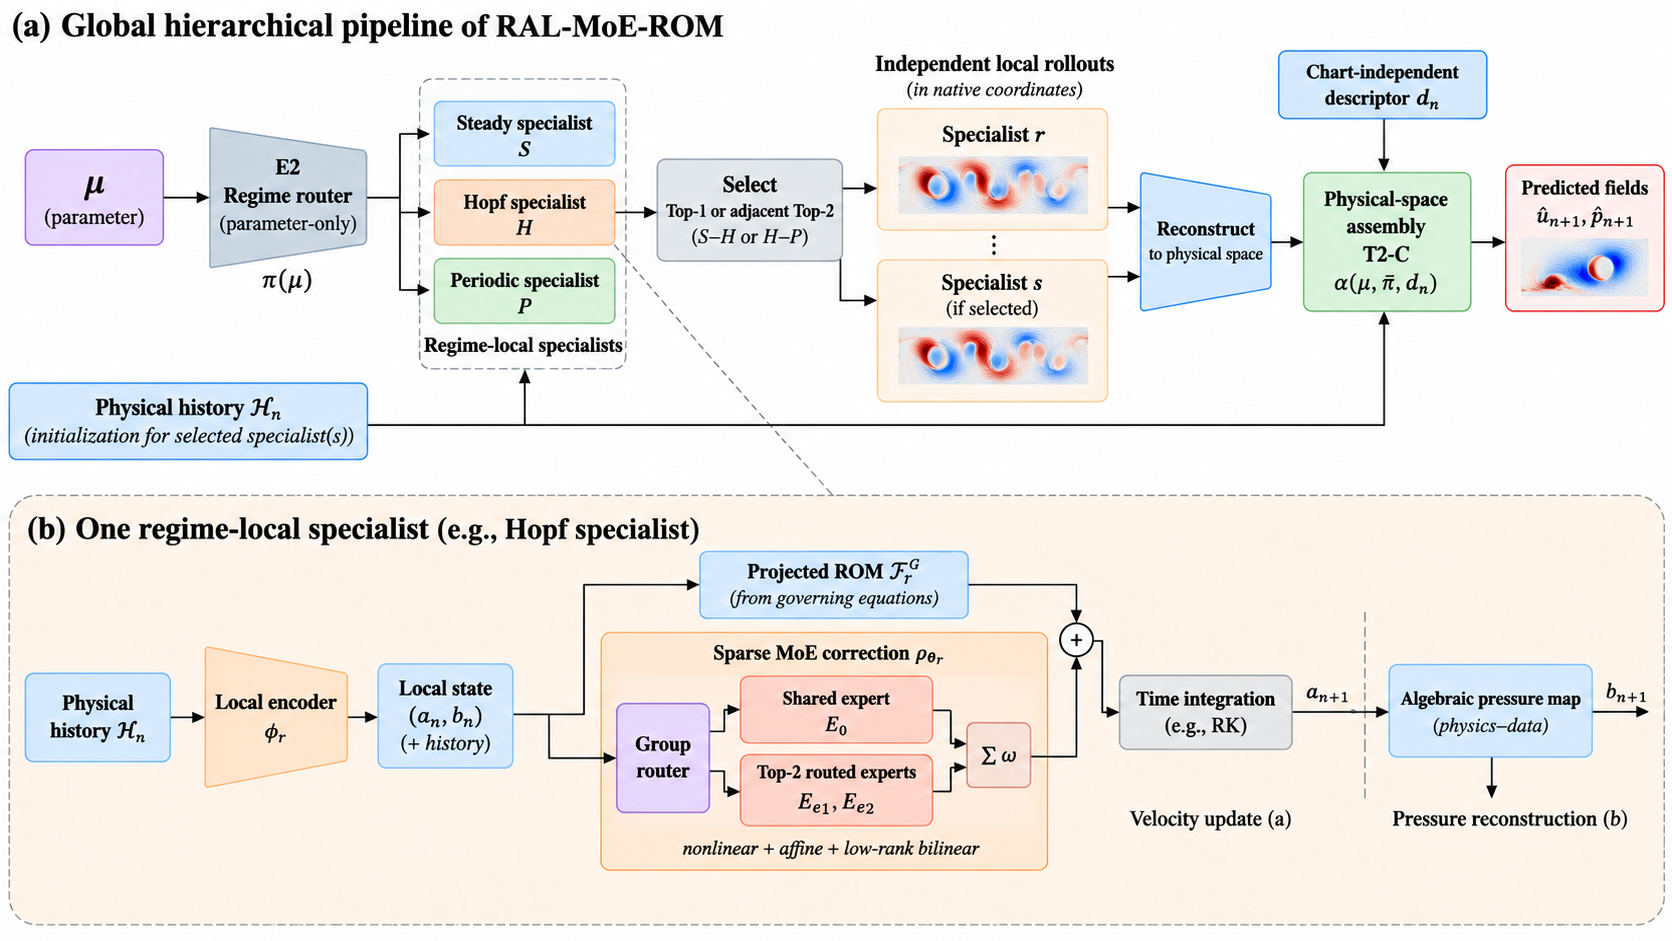
\includegraphics[width=\linewidth]{figures/ral_moe_rom_overview_user_20260908.png}
    \caption{Hierarchical routing in RAL-MoE-ROM.
    (a) Parameter-only E2 selects one specialist or an admissible adjacent pair.
    Physical history initializes native charts and supplies T2-C's descriptor
    $\bm d_n$ (history-to-assembly line), not E2. Independent rollouts are
    reconstructed before Top-1 identity output or Top-2 physical-space fusion,
    without fused-state feedback.
    (b) Within the selected group, shared and Top-2 experts contribute in parallel.
    Only velocity is integrated; pressure is reconstructed algebraically from
    updated velocity and local features (auxiliary connection omitted).
    Flow thumbnails are schematic, not experimental results.}
    \label{fig:ral_overview}
\end{figure}

We evaluate RAL-MoE-ROM on three parameterized incompressible-flow systems spanning
steady, Hopf-onset, and periodic dynamics. The experiments separate the effects of the
structured expert map, projected backbone, localization, and cross-regime assembly. Over
the evaluated finite horizons, the local specialists remain accurate and finite, and
T2-C improves the corresponding hard or single-specialist prediction in the tested
overlaps. The comparisons include vanilla experts, data-only dynamics, a global chart,
POD--Galerkin, one-step POD--DeepONet, hard routing, and fixed or probability-based
blends. Localization is not uniformly superior to a global model at every parameter;
its value emerges from combining local coordinates, regime-specific dynamics, and
adaptive assembly.

\section{Related Work}

\paragraph{Projection, learned dynamics, and autonomous rollout.}
POD--Galerkin methods project governing equations onto a data-adapted basis and retain an
interpretable reduced vector field \citep{sirovich1987,berkooz1993,benner2015}. Their
long-horizon accuracy can be limited by truncated scales, imperfect closure, and reduced
model stabilization \citep{amsallem2012}. Non-intrusive models instead learn reduced or
latent dynamics \citep{hesthaven2018,lee2020,champion2019,park2024}, and autoregressive
forecasters demonstrate the expressivity of learned evolution laws for complex temporal
systems \citep{pathak2018,vlachas2018}. Neural operators learn maps between function
spaces \citep{lu2021,kovachki2023}, whereas hybrid ROMs retain physical or projection
structure while learning unresolved components
\citep{duraisamy2019,brunton2020,dar2023,fresca2022,geelen2023}. RAL-MoE-ROM follows the
hybrid view, but replaces a single residual map with a conditionally sparse correction
trained under closed-loop rollout. This distinction is important because low one-step
error alone does not establish reliable recursive prediction.

\paragraph{Localized representations and conditional dynamics.}
Local reduced bases, operator localization, clustering, and nonlinear local manifolds
reduce the representational burden imposed on a single global chart
\citep{amsallem2008,peherstorfer2014,kaiser2014,li2021cluster,diaz2024}. These approaches
motivate parameter-local representations, but localization also makes the dynamics
chart dependent: independently constructed models generally differ in their means,
bases, scaling, and operators. RAL-MoE-ROM treats each chart as a complete autonomous
specialist and does not assume that two local coefficient vectors are commensurate. Its
cross-regime problem is therefore not merely basis selection; it is conditional assembly
of independently evolved dynamical systems.

\paragraph{Mixture-of-experts and the cross-chart gap.}
Classical hierarchical mixtures learn conditional expert assignments
\citep{jacobs1991,jordan1994}, and sparse MoE architectures scale conditional computation
by activating only a subset of experts \citep{shazeer2017,fedus2022}. Many MoE formulations
route predictors or operator blocks within a shared representation or common output space.
Recent work extends this specialization to decomposed hard physical constraints
\citep{ICLR2024_9aeda582}, local implicit representations
\citep{NEURIPS2024_b83fae17}, shared and routed experts for neural-operator pretraining
(MoE-POT; \citealt{NEURIPS2025_2d23a999}), and operator experts with parameter-conditioned
fusion for invariant PDE forecasting (iMOOE; \citealt{ICLR2026_754612bd}). These methods
specialize constraints, representations, or operator computations.
RAL-MoE-ROM instead places routing at two dynamical levels. Inside a local chart, group and channel routers activate
structured closure experts that share the same reduced coordinates. Outside the chart,
the E2 router selects complete autonomous projected ROM specialists whose reduced
coordinates are independently constructed.
An admissible adjacent pair is never averaged in coefficient space: both models roll out
independently and T2-C fuses only their reconstructed physical fields. This separation of
within-chart conditional closure from cross-chart dynamical assembly is the central gap
addressed here.

\section{RAL-MoE-ROM}
\label{sec:method}

RAL-MoE-ROM combines three operations within a two-level routing hierarchy.
Overlapping regime-local charts provide independent reduced representations.
Each chart carries a complete autonomous physics--data specialist whose projected
dynamics are corrected by a structured sparse MoE. The outer hierarchy selects one
specialist or an admissible adjacent pair and assembles only their reconstructed
physical fields. Figure~\ref{fig:ral_overview} summarizes the algorithm; full
derivations remain in Appendices~\ref{app:problem_pod}--\ref{app:routing}.

\subsection{Overlapping regime-local reduced charts}

Let $r\in\{S,H,P\}$ index steady, Hopf-onset, and periodic regimes, and let
$\mathcal M_r$ denote overlapping parameter regions. A physical velocity field is
encoded and reconstructed as
\begin{equation}
  \bm a^{(r)}={\Phi_u^{(r)}}^{\top}M_u(\bm u-\bar{\bm u}^{(r)}),\qquad
  \widehat{\bm u}^{(r)}=\bar{\bm u}^{(r)}+\Phi_u^{(r)}\bm a^{(r)},
  \label{eq:main_chart}
\end{equation}
where $M_u$ is the finite-volume quadrature matrix, with an analogous map for
gauge-fixed pressure coefficients $\bm b^{(r)}$. A complete chart contains its
parameter region, affine means, velocity and pressure bases, local normalization
statistics, and projected operators. These quantities are constructed independently
for each regime: equal reduced dimensions do not imply corresponding coordinates.
This is the reason cross-regime fusion is deferred to physical space.

\subsection{Physics--data specialists with structured sparse experts}

Projection supplies a regime-local dynamical backbone,
\begin{equation}
  \dot{\bm a}^{(r)}=
  \underbrace{\bm c_r+\bm A_r\bm a^{(r)}+
  \bm H_r:\bigl(\bm a^{(r)}\otimes\bm a^{(r)}\bigr)+
  \bm C^p_r\bm b^{(r)}}_{\mathcal F_r^{G}(\bm a^{(r)},\bm b^{(r)};\mu)}
  +\bm\rho^u_{\theta_r}(\bm\xi^{(r)}).
  \label{eq:main_specialist}
\end{equation}
The feature vector $\bm\xi^{(r)}$ contains standardized local coordinates, the projected right-hand side, the parameter, and a short state history. Channel-wise sparse MoEs parameterize the velocity closure $\bm\rho^u_{\theta_r}$ and learned pressure candidate $\bm\rho^p_{\theta_r}$,
\begin{equation}
  \begin{aligned}
  \mathcal M^c_{\theta_r}(\bm\xi)&=
  \omega^c_0 E^c_{0,g^\star}(\bm\xi)+
  \sum_{e\in\mathcal T_2^c}\omega^c_e E^c_{e,g^\star}(\bm\xi),\\
  E(\bm\xi)&=N(\bm\xi)+W_{\rm lin}\bm\xi+
  \kappa W_o\bigl[(U^\top\bm\xi)\odot(V^\top\bm\xi)\bigr].
  \end{aligned}
  \label{eq:main_inner_moe}
\end{equation}
The group router selects a chart-local expert family $g^\star$; velocity and pressure channels
$c\in\{u,p\}$ then use separate Top-2 subsets $\mathcal T_2^c$ together with the
always-active shared expert. The weights $\omega_e^c$ are nonnegative and sum to one
over these active experts. In the expert map, $N$ is the nonlinear branch, $\kappa$
scales the bilinear branch, and $\odot$ denotes componentwise multiplication.
The nonlinear, affine, and low-rank bilinear branches
provide complementary corrections without removing the projected backbone.
After each velocity macro-step, pressure is reconstructed algebraically as
\begin{equation}
  \bm b_{n+1}^{(r)}
  =\bm\gamma_n^{(r)}\odot\mathcal Q_r^{PP}(\bm a_{n+1}^{(r)};\mu)
  +\bigl(\bm 1-\bm\gamma_n^{(r)}\bigr)
   \odot\bm\rho^p_{\theta_r}(\bm\xi_n^{(r)}).
  \label{eq:main_pressure_closure}
\end{equation}
Here $\mathcal Q_r^{PP}$ is the chart-local pressure--Poisson map,
$\bm\rho^p_{\theta_r}$ supplies the learned pressure candidate, and
$\bm\gamma_n^{(r)}=\operatorname{sigmoid}(\bm\eta^p_{\theta_r}(\bm\xi_n^{(r)}))$
is a componentwise gate. Velocity is evolved differentially; pressure is recovered
by this semi-explicit algebraic closure, not a separate recurrent ODE.

\subsection{Closed-loop autonomous training}

Starting from encoded physical history, each specialist recursively consumes its own
predictions. For a window of length $K$, it minimizes the normalized coefficient loss
\begin{equation}
  \mathcal L_r=\frac{1}{K}\sum_{k=1}^{K}\left[
  \frac{\left\|(\widehat{\bm a}_{n+k}^{(r)}-\bm a_{n+k}^{(r)})
  \oslash\bm\sigma_a^{(r)}\right\|_2^2}{d_u}
  +\frac{\left\|(\widehat{\bm b}_{n+k}^{(r)}-\bm b_{n+k}^{(r)})
  \oslash\bm\sigma_b^{(r)}\right\|_2^2}{d_p}\right].
  \label{eq:main_rollout_loss}
\end{equation}
Here $d_u,d_p$ are the local coordinate dimensions and $\bm\sigma_a^{(r)},
\bm\sigma_b^{(r)}$ are training-population scaling vectors; $\oslash$ denotes
componentwise division. No reference state within the prediction window is injected
after initialization. The integrator and horizon curriculum are given in
Appendix~\ref{app:specialists}; held-out trajectory partitions are in
Table~\ref{tab:chart_splits}.

\subsection{Regime routing and physical-space T2-C fusion}

The outer E2 router depends only on the standardized physical parameter $\widetilde\mu$ and produces a trajectory-level regime preference $\bm\pi(\mu)=\operatorname{softmax}(\mathcal R_{E2}(\widetilde\mu))$. Its probabilities are evaluated once and remain fixed during the rollout. Chart-independent descriptors extracted from the initial physical history $\mathcal H_n$ are used only by the T2-C correction gate in an admissible overlap; they are not E2 inputs.
A binary mask $m_r(\mathcal H_n,\mu,K)$ excludes specialists whose
parameter--history pair or rollout horizon is outside the validation-supported
region. It constrains the candidate set, not the
E2 probability model. Hard Top-1 advances the largest-probability admissible specialist.
When an adjacent pair is admissible ($S$--$H$ or $H$--$P$), both specialists encode the same physical history in their native coordinates and then evolve independently. For reconstructed fields $\widehat{\bm q}^{(r)}$ and $\widehat{\bm q}^{(s)}$, T2-C predicts a window-conditioned convex weight and forms
\begin{equation}
  \widehat{\bm q}_{\rm T2C}(t)
  =\alpha\,\widehat{\bm q}^{(r)}(t)+(1-\alpha)\,\widehat{\bm q}^{(s)}(t),
  \qquad \alpha=\sigma\!\left(\operatorname{logit}(\bar\pi_r)+\Delta_\psi\right).
  \label{eq:main_t2c}
\end{equation}
Here $\bm q$ collects velocity and gauge-fixed pressure on the common mesh, and
$\sigma$ is the sigmoid. One scalar $\alpha$ is fixed throughout the window and
shared by both fields. The pair-normalized E2 probability is $\bar\pi_r$, and
$\Delta_\psi=c_\psi([\widetilde\mu;\bm d_n])$ is a learned correction based on the
standardized parameter and chart-independent physical-history descriptor $\bm d_n$.
Fusion occurs after reconstruction and is not fed back into either local rollout.
No prediction is asserted if all masks are zero. Admissibility is selected from
validation support and should not be interpreted as a formal stability certificate.

\section{Experiments}
\label{sec:experiments}

We evaluate the two levels of RAL-MoE-ROM through complementary benchmark roles.
All three two-dimensional incompressible-flow datasets span steady, Hopf-onset,
and periodic dynamics as the Reynolds number varies. The circular-cylinder
benchmark provides the local-specialist ablation, the centered-square benchmark
provides matched $S$--$H$ and $H$--$P$ routing/fusion comparisons, and the
fluidic-pinball benchmark provides the autonomous comparison with a classical
POD--Galerkin baseline. Table~\ref{tab:benchmark_summary} summarizes this scope.
All training, validation, and test partitions are defined by complete parameter
trajectories; chart-wise ranges and split counts are reported in
Appendix~\ref{app:implementation}.

Errors $E_u$ and $E_p$ are relative physical-field errors in percent
(Appendix~\ref{app:implementation}), aggregated
according to each benchmark's evaluation protocol; $E_{\mathrm{joint}}=E_u+E_p$.
The sum of displayed component errors can differ slightly from the reported
joint error because values are rounded independently.
``Divergent'' denotes an evaluation window that violates the predefined
rollout-divergence criterion, including non-finite states or threshold
violations. N/E denotes not evaluable under the prescribed rollout criterion;
table-specific notes give the reason.

\begin{table}[t]
\centering
\caption{Experimental scope. Local rank pairs $(r_u,r_p)$ and horizons are ordered $S,H,P$;
$K$ counts rollout steps at each benchmark's sampling interval. Additional
overlap and periodic-core settings are specified in their comparisons.}
\label{tab:benchmark_summary}
\small
\setlength{\tabcolsep}{4pt}
\begin{tabular}{@{}>{\raggedright\arraybackslash}p{2.15cm}
>{\raggedright\arraybackslash}p{1.30cm}
>{\raggedright\arraybackslash}p{4.05cm}
>{\raggedright\arraybackslash}p{1.80cm}
>{\raggedright\arraybackslash}p{2.50cm}@{}}
\toprule
Benchmark & $Re$ range & Local ranks ($S,H,P$) & Main horizons & Primary role \\
\midrule
Circular cylinder & 20--200 & $(32,32),\ (32,32),\ (32,32)$ & $56/56/48$ & Local specialist ablation \\
\addlinespace
Centered square & 50--150 & $(5,4),\ (11,11),\ (28,26)$ & $16/48/24$ & Routing and fusion \\
\addlinespace
Fluidic pinball & 10--60 & $(4,3),\ (5,5),\ (17,16)$ & $56/56/32$ & Autonomous baseline \\
\bottomrule
\end{tabular}
\end{table}

\subsection{Do local specialists support long autonomous rollouts?}

The learned fluidic-pinball specialists complete all four evaluation settings
without violating the prescribed rollout-divergence criterion, whereas
POD--Galerkin violates the criterion in all 448 Steady windows and in
141 of 320 Hopf windows (Table~\ref{tab:pinball_autonomous}).
The component errors reveal a substantially larger pressure discrepancy for
POD--Galerkin in the evaluable Hopf and Periodic settings. The learned
specialists support autonomous prediction over the evaluated finite horizons.
The circular-cylinder ablation and centered-square local-specialist results
provide complementary evidence in Table~\ref{tab:compact_ablation} and
Appendix~\ref{app:square}, respectively.

\begin{table}[t]
\centering
\caption{Autonomous local-specialist prediction on the fluidic-pinball benchmark.
Errors are percentages; lower is better. Periodic core ($K=56$) denotes the
longer-horizon stride-four matched final-test evaluation within the periodic
regime; complete cadence details are given in Appendix~\ref{app:pinball}.}
\label{tab:pinball_autonomous}
\small
\setlength{\tabcolsep}{5pt}
\begin{threeparttable}
\begin{tabular}{@{}llrrr@{}}
\toprule
Evaluation setting & Model & $E_u$ & $E_p$ & $E_{\mathrm{joint}}$ \\
\midrule
Steady ($K=56$) & POD--Galerkin & N/E$^\dagger$ & N/E$^\dagger$ & N/E$^\dagger$ \\
 & RAL-MoE-ROM & 0.2247 & 0.7593 & 0.9840 \\
\addlinespace
Hopf ($K=56$) & POD--Galerkin & 0.4378$^\ddagger$ & 48.50$^\ddagger$ & 48.94$^\ddagger$ \\
 & RAL-MoE-ROM & 0.0995 & 1.986 & 2.085 \\
\addlinespace
Periodic ($K=32$) & POD--Galerkin & 1.641 & 41.56 & 43.20 \\
 & RAL-MoE-ROM & 0.2897 & 0.5518 & 0.8415 \\
\addlinespace
Periodic core ($K=56$) & POD--Galerkin & 2.555 & 39.36 & 41.91 \\
 & RAL-MoE-ROM & 0.6222 & 1.050 & 1.672 \\
\bottomrule
\end{tabular}
\begin{tablenotes}[flushleft]
\footnotesize
\item[$\dagger$] All 448 evaluation windows violate the predefined rollout-divergence criterion.
\item[$\ddagger$] Errors are computed for all numerically finite windows;
141 of 320 Hopf windows exceed the predefined rollout-divergence threshold.
All RAL-MoE-ROM settings and both periodic POD--Galerkin settings have zero divergent windows.
\end{tablenotes}
\end{threeparttable}
\end{table}

\noindent A complementary global POD--DeepONet baseline illustrates the
distinction between one-step fitting and autonomous prediction: it achieves
$E_u=1.5921\%$ and $E_p=23.3447\%$ on 4,228 held-out one-step pairs, yet
only one of 28 held-out trajectories remains finite under recursive rollout.
Its cadence differs from the matched Periodic specialist evaluation, so this
is a one-step versus recursive-stability contrast, not a matched long-horizon
accuracy comparison (Appendix~\ref{app:pinball}).

\subsection{Does learned physical-space fusion improve overlap prediction?}

To isolate the second routing level, we compare centered-square $S$--$H$ and
$H$--$P$ overlaps at $K=24$ (Table~\ref{tab:routing_fusion}). Alongside hard
routing, equal and E2-probability blends, and the diagnostic oracle, we include
T2-C $\mu$-only: the same correction network and optimization protocol with all
standardized history-descriptor channels set to zero. This preserves the gate
architecture and parameter count while removing history information.

Parameter-only correction behaves differently across overlaps: in $S$--$H$ it
remains close to E2-probability blending ($2.1846\%$ versus $2.1847\%$), whereas
in $H$--$P$ it improves the blend ($1.1504\%$ versus $1.6618\%$).
History conditioning provides an additional gain in both, yielding
$1.1958\%$ and $0.8465\%$. Full T2-C reduces joint error by $30.9\%/29.9\%$
relative to the best fixed specialist and $30.9\%/54.2\%$ relative to E2 Top-1
($S$--$H$/$H$--$P$), and remains close to the diagnostic convex oracle.
Figure~\ref{fig:square_overlap} shows representative fields and velocity errors.

Across three paired gate-training seeds, full T2-C outperforms the
architecture-matched $\mu$-only gate in all runs for both overlaps, with mean
joint-error reductions of $45.3\%$ on $S$--$H$ and $26.2\%$ on $H$--$P$.
Full T2-C gives
$E_{\mathrm{joint}}=1.1957\pm0.0001\%$ on $S$--$H$ and
$0.8500\pm0.0035\%$ on $H$--$P$ (sample standard deviation across gate-training seeds).
Only the gate is retrained; specialists, E2, candidate rollouts, partitions,
normalization, and optimization protocol are fixed. Component and seed-wise
results are in Appendix~\ref{app:square}; the fluidic-pinball overlap study is
in Appendix~\ref{app:pinball}.

\begin{table}[t]
\centering
\caption{Fixed-run cross-regime routing and fusion on the centered-square benchmark at
$K=24$. Entries are terminal-step $E_{\mathrm{joint}}$ (\%); lower is better.
T2-C $\mu$-only zeroes the standardized history channels in the same gate architecture.
The convex oracle is an a posteriori convex reference unavailable during prediction;
three-seed gate variability is reported separately in Appendix~\ref{app:square}.
Bold marks the best deployable assembly in this fixed-run comparison.}
\label{tab:routing_fusion}
\small
\setlength{\tabcolsep}{3.5pt}
\begin{threeparttable}
\begin{tabular}{@{}lrrrrrrr@{}}
\toprule
Overlap & Best single$^\ast$ & E2 Top-1 & Equal & E2 prob. & T2-C $\mu$-only & T2-C & Oracle \\
\midrule
$S$--$H$ & 1.7298 & 1.7298 & 3.0321 & 2.1847 & 2.1846 & \textbf{1.1958} & 1.1842 \\
$H$--$P$ & 1.2079 & 1.8473 & 1.6146 & 1.6618 & 1.1504 & \textbf{0.8465} & 0.8384 \\
\bottomrule
\end{tabular}
\begin{tablenotes}[flushleft]
\footnotesize
\item[$\ast$] Best single is an a posteriori fixed-specialist reference selected
by aggregate evaluation error over the corresponding overlap (Hopf for $S$--$H$,
Periodic for $H$--$P$); it is not a routing strategy available during prediction.
\end{tablenotes}
\end{threeparttable}
\end{table}

\begin{figure}[t]
\centering
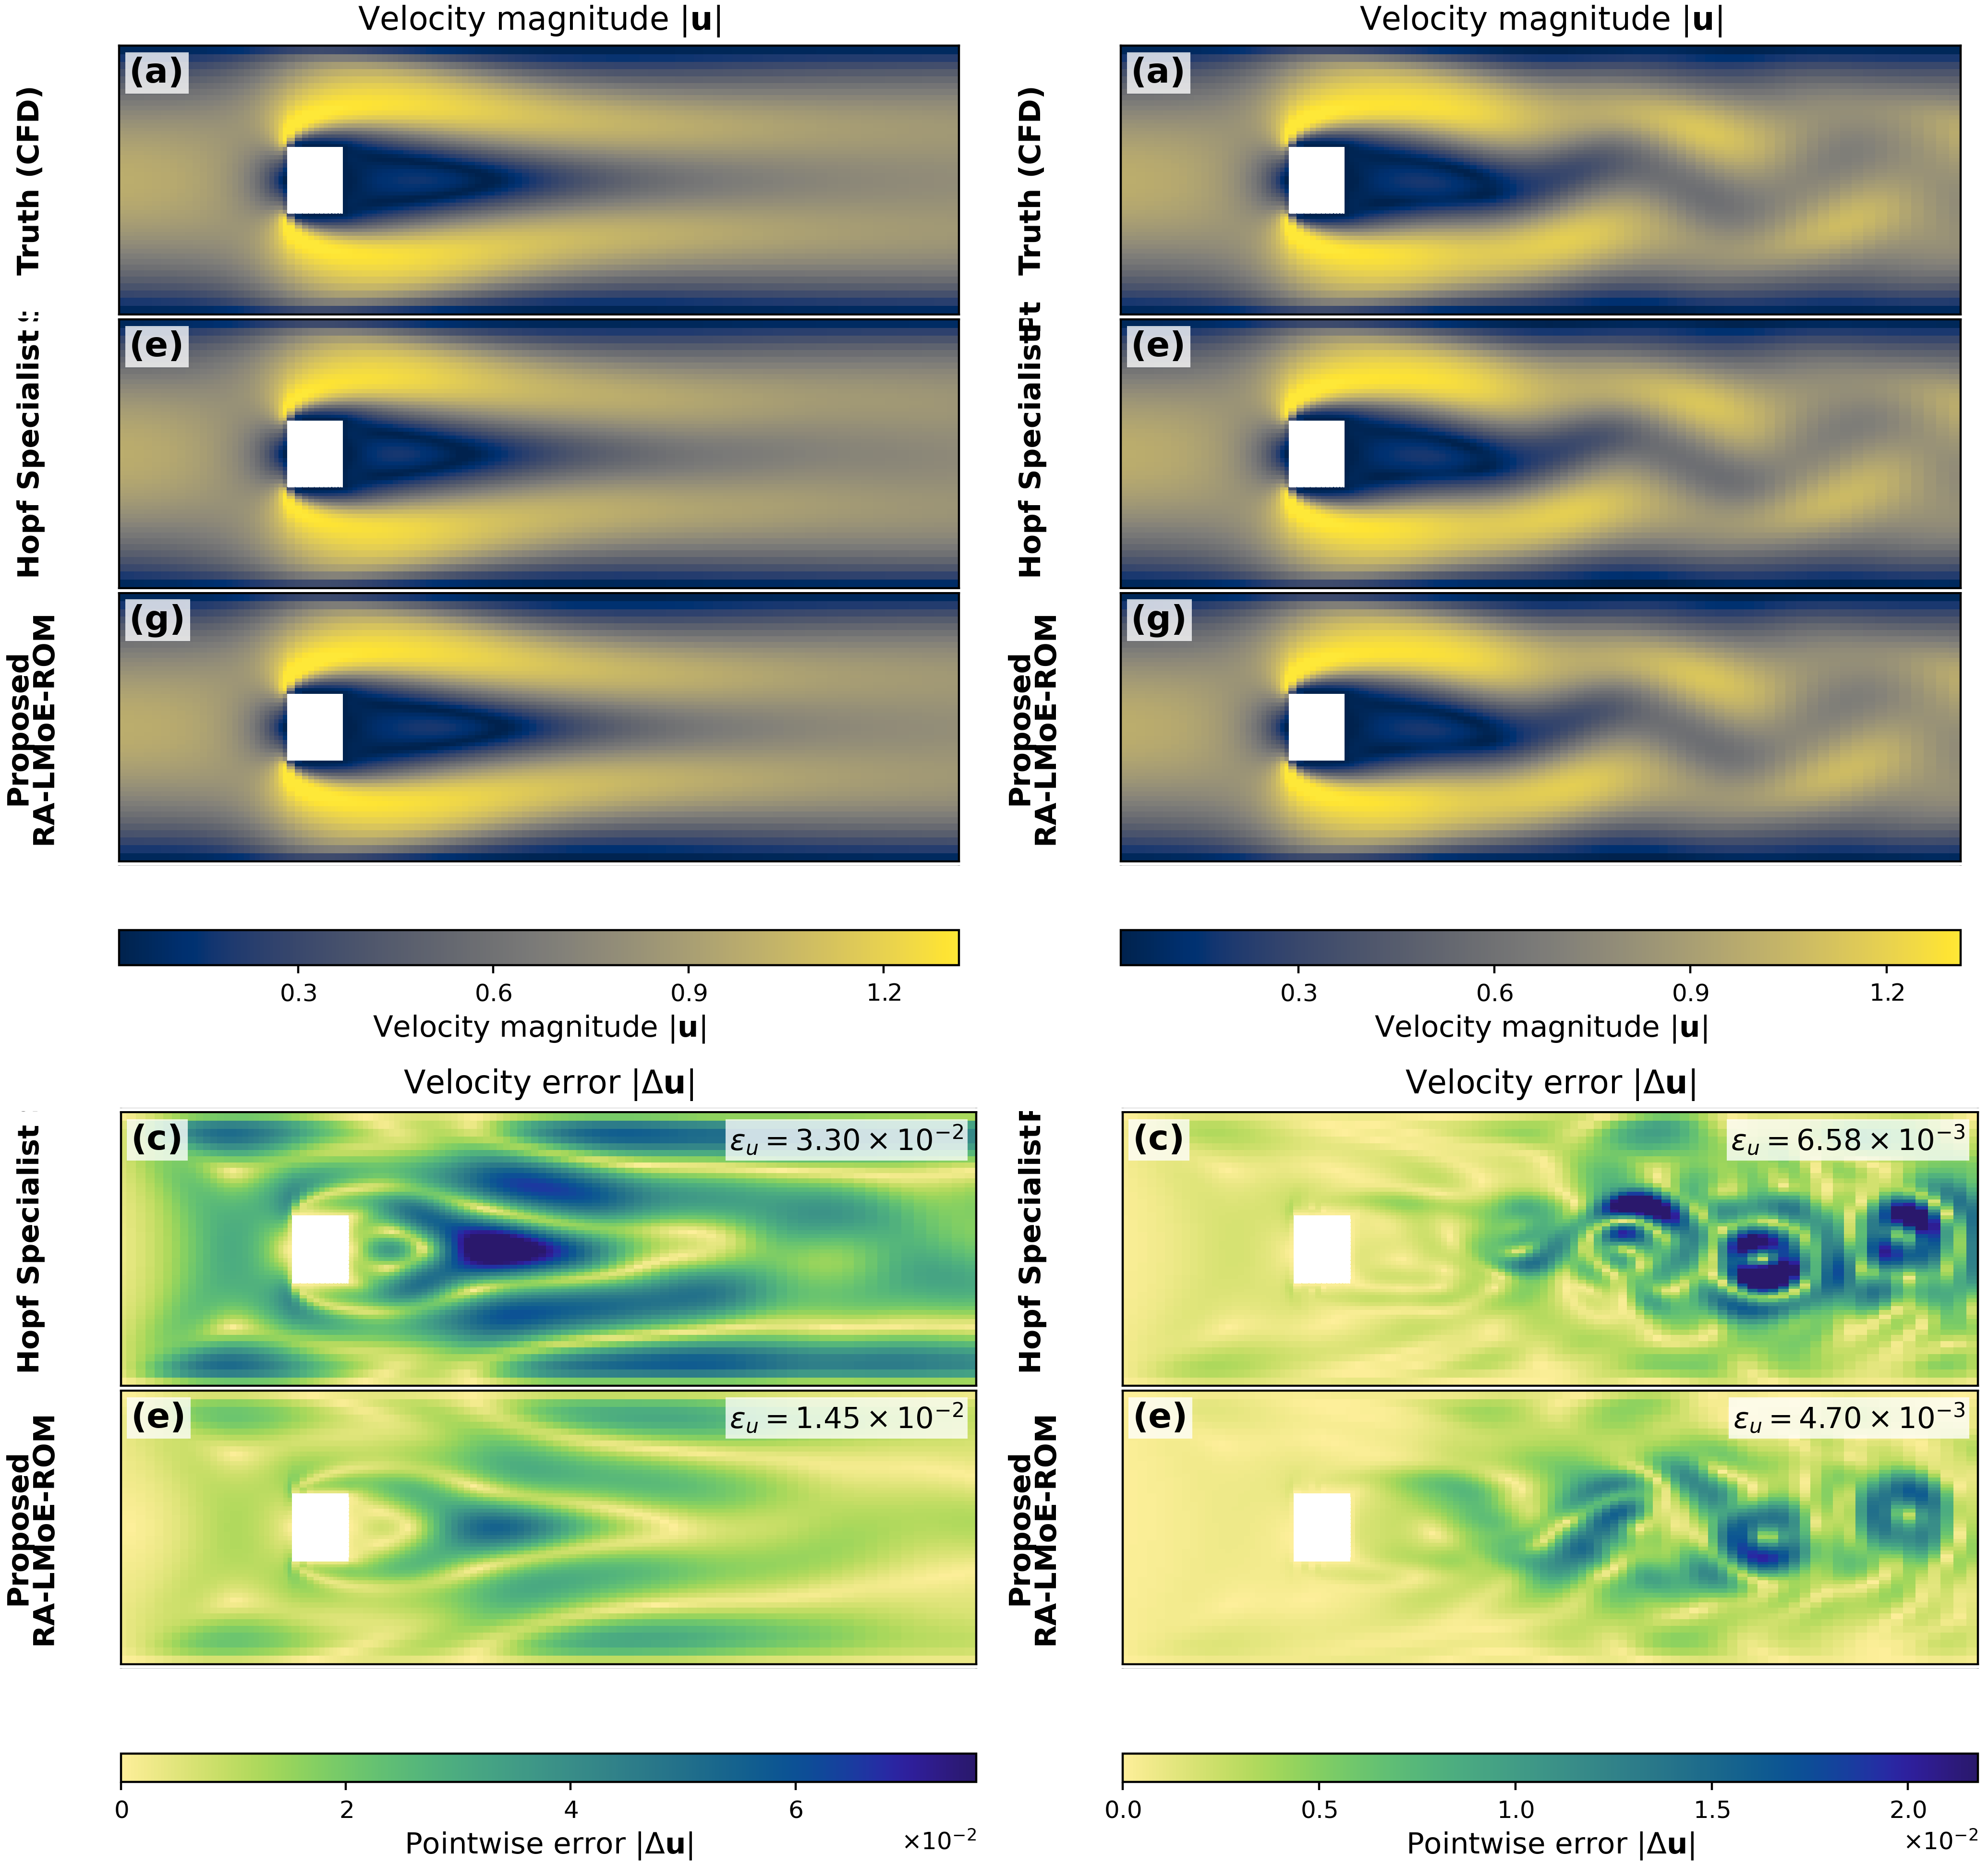
\includegraphics[width=\linewidth]{figures/square_overlap_compact.png}
\caption{Centered-square $S$--$H$ (left) and $H$--$P$ (right) overlap predictions.
T2-C fuses independently evolved, reconstructed fields and reduces velocity-field
discrepancy relative to the corresponding single specialist. Complete velocity
and pressure fields appear in Appendix~\ref{app:square}.}
\label{fig:square_overlap}
\end{figure}

\subsection{What do local architectural components contribute?}

The circular-cylinder comparison probes the contributions of three local modeling choices
(Table~\ref{tab:compact_ablation}). Vanilla-FNN-MoE replaces the structured
expert map with conventional feed-forward experts, DataOnly-MoE removes the
projected Galerkin and Pressure--Poisson contributions, and Global MoE replaces
the local charts and specialists with one global model. The comparison uses
physical-field errors so that models with different reduced coordinates can
be evaluated on a common quantity.
These comparisons probe architectural effects under the available fixed models;
they are not parameter-matched capacity controls.
Total and per-decision active trainable parameter counts for the analyzed
Hopf and Periodic specialists are reported in Appendix~\ref{app:parameter_counts}.

\begin{table}[!ht]
\centering
\caption{Local architecture ablation on the circular-cylinder benchmark.
Each regime cell reports the min--max $E_u$ range (upper line) and $E_p$
range (lower line) over held-out Reynolds-number trajectories, in percent.
These are field-error ranges, not means or uncertainty intervals.
N/E denotes not evaluable under the prescribed rollout criterion: the
Vanilla-FNN-MoE Hopf model does not meet the validation-stage stability
requirement and is not evaluated on held-out trajectories.}
\label{tab:compact_ablation}
\small
\setlength{\tabcolsep}{4pt}
\begin{tabular}{@{}lccc@{}}
\toprule
Model & Steady ($K=56$) & Hopf ($K=56$) & Periodic ($K=48$) \\
\midrule
RAL-MoE-ROM
& \shortstack{0.0330--0.1723\\0.2500--1.3249}
& \shortstack{0.0032--0.0288\\0.0355--0.4321}
& \shortstack{0.3809--1.3473\\1.6825--5.9601} \\
\addlinespace
Vanilla-FNN-MoE
& \shortstack{0.0384--0.2995\\2.2163--18.5603}
& N/E
& \shortstack{1.0393--3.0836\\3.9659--13.3257} \\
\addlinespace
DataOnly-MoE
& \shortstack{0.1637--0.5122\\4751.1025--27275.4645}
& \shortstack{0.1260--0.3880\\1280.2811--1524.5949}
& \shortstack{0.7854--1.8677\\2.2511--10.8189} \\
\addlinespace
Global MoE
& \shortstack{0.0845--0.3404\\1.5226--7.4363}
& \shortstack{0.0110--0.0268\\0.0560--0.2882}
& \shortstack{0.5873--1.1726\\2.1896--6.3566} \\
\bottomrule
\end{tabular}
\end{table}

\FloatBarrier
Structured specialists improve the steady and periodic error ranges over
Vanilla-FNN-MoE, which does not meet the validation-stage stability requirement
for the Hopf evaluation. Removing the physical backbone
particularly degrades steady and Hopf pressure prediction. The global model
remains competitive in Hopf and periodic physical-field errors, so
localization is not uniformly superior; its role is to provide regime-specific
coordinates and dynamics that can participate in cross-regime assembly.
The local comparisons address expert structure, physics, and localization,
while Table~\ref{tab:routing_fusion} separately evaluates the outer assembly.

\paragraph{Internal routing behavior.}
Post-hoc analysis of the circular-cylinder Periodic specialist shows conditional
use of the Level-1 sparse experts (Figure~\ref{fig:periodic_internal_routing}).
Across held-out autonomous rollouts, sampled once per macro-step, the velocity
channel uses all 18 routed experts through 33 distinct group/pair configurations,
while the pressure channel uses 14 of 18 experts through 16 configurations.
Group allocation changes across the four held-out Reynolds
numbers, and the channels exhibit distinct routing profiles. This diagnostic
supports conditional expert utilization, not physical semantics for individual
experts; the contrasting Hopf profile is reported in
Appendix~\ref{app:internal_routing}.

\begin{figure}[!ht]
\centering
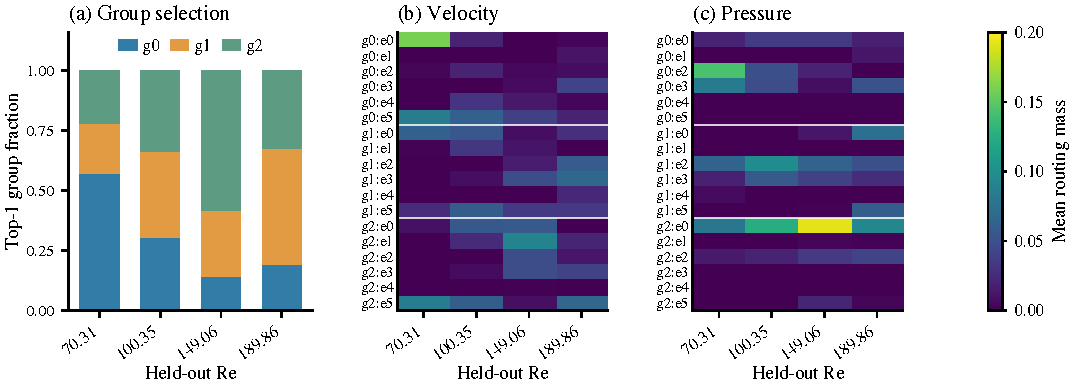
\includegraphics[width=\linewidth]{figures/periodic_internal_routing.pdf}
\caption{Internal routing of the circular-cylinder Periodic specialist on
held-out autonomous rollout windows, with one record per macro-step at the
first integration stage.
(a) Top-1 group-selection fractions. (b,c) Mean routed-expert mass for velocity
and pressure. Expert IDs are local to the specialist, channel, and group;
they do not denote physical mechanisms.}
\label{fig:periodic_internal_routing}
\end{figure}

\FloatBarrier
\section{Limitations}

The regime cover and admissible adjacency graph are selected using validation support;
the method does not discover arbitrary bifurcation structure or certify unseen
transitions. T2-C is evaluated only between adjacent specialists, and convex
physical-space fusion may be insufficient when more than two regimes interact or when
conserved quantities require a constrained assembly rule. The evidence concerns
two-dimensional incompressible flows and empirical finite-horizon behavior; it does not
establish provable stability, conservation, or accuracy outside the sampled parameter
ranges. A separate hierarchy is trained for each benchmark, so cross-geometry transfer
of one hierarchy is not evaluated. Multiple local bases, operators, and specialists also
increase training and model-management cost relative to one global ROM.

Repeated-seed variability is evaluated for the T2-C correction gate with local
specialists, E2, and data partitions held fixed. A full multi-seed study of the
regime-local specialists and complete hierarchy, and parameter-matched capacity
comparisons of the local models, remain future work.
The internal-routing analysis is descriptive: it does not establish a unique
physical interpretation or a causal performance contribution for individual
experts, nor does it imply equally rich expert switching in every chart.

\section{Conclusion}

RAL-MoE-ROM casts broad-parameter reduced dynamics as a two-level mixture-of-experts problem. Structured sparse experts learn unresolved dynamics inside each physics--data specialist, while an outer router selects or combines complete local models. Keeping the local coordinates independent and coupling only reconstructed physical fields avoids interpolation between incompatible modal states. Across the three evaluated flow systems, the specialists achieve low error over the evaluated autonomous rollout horizons, and T2-C improves prediction in the tested transition regions. The results motivate extensions that learn the regime cover, impose physical constraints on field-space fusion, and evaluate the hierarchy on higher-dimensional and non-fluid dynamical systems.


\subsubsection*{Reproducibility statement}
The main text reports the benchmark roles, evaluation horizons, baselines, and metrics. Appendices~A--E document the local-coordinate construction, projected operators, specialist architecture, routing and fusion procedure, and implementation details. Appendices~F--H provide benchmark-specific results.
Appendix~\ref{app:internal_routing} reports post-hoc internal-routing statistics
from fixed validation-selected Hopf and Periodic specialists on held-out
rollout windows; these diagnostics are not used for model selection.
Appendix~\ref{app:square} additionally reports an architecture-matched descriptor
ablation and three-seed variability of the centered-square T2-C gate, with the
underlying specialists and E2 router held fixed.

\subsection*{AI use statement}
% Authors must confirm this disclosure against the final submission workflow.
Generative AI tools, including ChatGPT and Codex, assisted with language editing,
LaTeX and code refactoring, analysis scripting and interpretation, literature
checks, and schematic figure preparation.
The authors take full responsibility for reviewing and verifying all scientific
content, mathematical formulations, experimental configurations, numerical
results, and conclusions, and for the final manuscript and all reported results.

\bibliography{references,legacy_references}
\bibliographystyle{iclr2027_conference}

\appendix
\section{Full problem setup and weighted POD construction}
\label{app:problem_pod}

\subsection{Parameterized full-order model, gauge, and regime cover}

After spatial discretization, the velocity $\bm u(t;\mu)\in\mathbb R^{N_u}$ and pressure $p(t;\mu)\in\mathbb R^{N_p}$ satisfy
\begin{equation}
 \dot{\bm u}=\bm f_h(\mu)+\mathcal L_h(\mu)\bm u
 -\mathcal N_h(\bm u,\bm u;\mu)-\nabla_h(\mu)p,
 \qquad \operatorname{div}_h(\mu)\bm u=0.
 \label{eq:app_fom}
\end{equation}
Pressure is defined only up to an additive constant. With positive finite-volume weights $\bm w$, every pressure snapshot is mapped to the weighted zero-mean gauge
\begin{equation}
 \Gamma_p(q)=q-\frac{\bm w^\top q}{\bm w^\top\bm 1}\bm 1,
 \qquad p^\circ=\Gamma_p(p),
 \qquad \bm w^\top p^\circ=0.
 \label{eq:app_pressure_gauge}
\end{equation}
The parameter domain is covered by overlapping regions
\begin{equation}
 \mathcal M\subseteq\bigcup_{r\in\{S,H,P\}}\mathcal M_r,
 \qquad \mathcal O_{SH}=\mathcal M_S\cap\mathcal M_H,
 \qquad \mathcal O_{HP}=\mathcal M_H\cap\mathcal M_P.
 \label{eq:app_regime_cover}
\end{equation}
No direct $S$--$P$ overlap is used.

\subsection{Area-weighted local POD}

The finite-volume quadrature induces
\begin{equation}
 \langle\bm v,\bm z\rangle_{M_u}=\bm v^\top M_u\bm z,
 \qquad \langle q,s\rangle_{M_p}=q^\top M_p s,
 \qquad M_p=\operatorname{diag}(\bm w),\quad M_u=\operatorname{diag}(M_p,M_p).
 \label{eq:app_weighted_inner_products}
\end{equation}
For chart $r$, let $X_u^{(r)}$ and $X_p^{(r)}$ contain velocity and gauge-corrected pressure snapshots after subtracting their chart-specific means $\bar{\bm u}^{(r)}$ and $\bar p^{(r),\circ}$. The local bases solve
\begin{align}
 \Phi_u^{(r)}&\in\underset{\Psi^\top M_u\Psi=I_{d_u}}{\operatorname{arg\,min}}
 \left\|X_u^{(r)}-\Psi\Psi^\top M_uX_u^{(r)}\right\|_{M_u,F}^2,\\
 \Phi_p^{(r)}&\in\underset{\Psi^\top M_p\Psi=I_{d_p}}{\operatorname{arg\,min}}
 \left\|X_p^{(r)}-\Psi\Psi^\top M_pX_p^{(r)}\right\|_{M_p,F}^2,
 \label{eq:app_pod_optimization}
\end{align}
where $\|Y\|_{M,F}^2=\operatorname{tr}(Y^\top MY)$. Equivalently, for the weighted singular value decompositions
\begin{equation}
 M_u^{1/2}X_u^{(r)}=U_u^{(r)}\Sigma_u^{(r)}{V_u^{(r)}}^\top,
 \qquad M_p^{1/2}X_p^{(r)}=U_p^{(r)}\Sigma_p^{(r)}{V_p^{(r)}}^\top,
\end{equation}
the bases are
\begin{equation}
 \Phi_u^{(r)}=M_u^{-1/2}U_u^{(r)}(:,1{:}d_u),
 \qquad \Phi_p^{(r)}=M_p^{-1/2}U_p^{(r)}(:,1{:}d_p),
 \label{eq:app_weighted_svd_bases}
\end{equation}
and satisfy ${\Phi_u^{(r)}}^\top M_u\Phi_u^{(r)}=I$ and ${\Phi_p^{(r)}}^\top M_p\Phi_p^{(r)}=I$. Gauge consistency also gives $\bm w^\top\Phi_p^{(r)}=\bm 0^\top$.

Encoding and decoding are chart specific:
\begin{align}
 \bm a^{(r)}&={\Phi_u^{(r)}}^\top M_u(\bm u-\bar{\bm u}^{(r)}),
 &\mathcal D_r^u(\bm a^{(r)})&=\bar{\bm u}^{(r)}+\Phi_u^{(r)}\bm a^{(r)},\\
 \bm b^{(r)}&={\Phi_p^{(r)}}^\top M_p(\Gamma_p(p)-\bar p^{(r),\circ}),
 &\mathcal D_r^p(\bm b^{(r)})&=\bar p^{(r),\circ}+\Phi_p^{(r)}\bm b^{(r)}.
 \label{eq:app_encode_decode}
\end{align}
Learned components use local standardizations
\begin{equation}
 \widetilde{\bm a}^{(r)}=(\bm a^{(r)}-\bm\mu_a^{(r)})\oslash\bm\sigma_a^{(r)},
 \qquad
 \widetilde{\bm b}^{(r)}=(\bm b^{(r)}-\bm\mu_b^{(r)})\oslash\bm\sigma_b^{(r)}.
 \label{eq:app_local_scalers}
\end{equation}

\section{Projected Galerkin and pressure operators}
\label{app:rom}

\subsection{Chart-local momentum dynamics}

Substituting the affine reconstructions into Eq.~(\plaineqref{eq:app_fom}) and testing against the local velocity basis gives
\begin{equation}
 \dot{\bm a}^{(r)}=\bm c_r(\mu)+A_r(\mu)\bm a^{(r)}
 +H_r(\mu):(\bm a^{(r)}\otimes\bm a^{(r)})+C_r^p(\mu)\bm b^{(r)}.
 \label{eq:app_projected_momentum}
\end{equation}
For velocity modes $\bm\phi_i^{u,(r)}$ and pressure modes $\phi_\ell^{p,(r)}$,
\begin{align}
 [\bm c_r]_i
 &=\left\langle\bm\phi_i^{u,(r)},
 \bm f_h+\mathcal L_h\bar{\bm u}^{(r)}
 -\mathcal N_h(\bar{\bm u}^{(r)},\bar{\bm u}^{(r)};\mu)
 -\nabla_h\bar p^{(r),\circ}\right\rangle_{M_u},\\
 [A_r]_{ij}
 &=\left\langle\bm\phi_i^{u,(r)},
 \mathcal L_h\bm\phi_j^{u,(r)}
 -\mathcal N_h(\bar{\bm u}^{(r)},\bm\phi_j^{u,(r)};\mu)
 -\mathcal N_h(\bm\phi_j^{u,(r)},\bar{\bm u}^{(r)};\mu)
 \right\rangle_{M_u},\\
 [H_r]_{ijk}
 &=-\left\langle\bm\phi_i^{u,(r)},
 \mathcal N_h(\bm\phi_j^{u,(r)},\bm\phi_k^{u,(r)};\mu)
 \right\rangle_{M_u},\\
 [C_r^p]_{i\ell}
 &=-\left\langle\bm\phi_i^{u,(r)},\nabla_h(\mu)\phi_\ell^{p,(r)}\right\rangle_{M_u}.
 \label{eq:app_projected_operators}
\end{align}
These terms define the backbone $\mathcal F_r^G(\bm a,\bm b;\mu)$ used in Eq.~(\plaineqref{eq:main_specialist}).

\subsection{Gauge-consistent pressure--Poisson map}

At the continuous level the gauge-fixed pressure satisfies
\begin{equation}
 -\Delta p^\circ=\nabla\!\cdot\!\left[(\bm u\!\cdot\!\nabla)\bm u-\bm f\right],
 \qquad \int_\Omega p^\circ\,\mathrm d\Omega=0,
\end{equation}
with boundary conditions inherited from the momentum equation. Projection of the discrete relation gives
\begin{equation}
 K_r^p(\mu)\bm b^{PP,(r)}=\bm d_r(\mu)+B_r(\mu)\bm a^{(r)}
 +Q_r(\mu):(\bm a^{(r)}\otimes\bm a^{(r)}),
 \label{eq:app_pressure_poisson_system}
\end{equation}
and hence
\begin{equation}
 \mathcal Q_r^{PP}(\bm a;\mu)=[K_r^p(\mu)]^{-1}
 \left[\bm d_r(\mu)+B_r(\mu)\bm a+Q_r(\mu):(\bm a\otimes\bm a)\right].
 \label{eq:app_pressure_poisson_map}
\end{equation}
The gauge removes the constant pressure nullspace. Each complete chart therefore contains its own parameter region, affine means, bases, scalers, $\mathcal F_r^G$, and $\mathcal Q_r^{PP}$. Equal reduced dimensions do not create a canonical componentwise identification between two charts; only decoded physical fields share a common representation.

\section{Specialist architecture and closed-loop objective}
\label{app:specialists}

Each regime-local chart is equipped with an independently parameterized
semi-explicit specialist. The velocity coefficients evolve under the sum of
the chart-local Galerkin vector field and a learned closure,
\begin{equation}
  \dot{\bm a}^{(r)}
  =
  \mathcal F_r^G\!\left(\bm a^{(r)},\bm b^{(r)};\mu\right)
  +\bm\rho^u_{\theta_r}\!\left(\bm\xi^{(r)}\right).
  \label{eq:app_hybrid_velocity_rhs}
\end{equation}
Pressure is algebraic rather than an independently evolved recurrent state.
After the velocity macro-step, the local pressure--Poisson operator provides
the physics-based candidate
\begin{equation}
  \bm b_{n+1}^{PP,(r)}
  =\mathcal Q_r^{PP}\!\left(\bm a_{n+1}^{(r)};\mu\right),
  \label{eq:app_pressure_poisson_candidate}
\end{equation}
while a data-driven candidate and a componentwise gate are evaluated from the
specialist feature vector,
\begin{align}
  \widehat{\bm b}_{n+1}^{D,(r)}
  &=\bm\rho^p_{\theta_r}\!\left(\bm\xi_n^{(r)}\right),
  &
  \bm\gamma_n^{(r)}
  &=\operatorname{sigmoid}\!\left(
      \bm\eta^p_{\theta_r}\!\left(\bm\xi_n^{(r)}\right)
    \right).
  \label{eq:app_pressure_candidates}
\end{align}
The next pressure state is the componentwise convex combination
\begin{equation}
  \bm b_{n+1}^{(r)}
  =\bm\gamma_n^{(r)}\odot\bm b_{n+1}^{PP,(r)}
  +\left(\bm 1-\bm\gamma_n^{(r)}\right)
   \odot\widehat{\bm b}_{n+1}^{D,(r)},
  \qquad \bm\gamma_n^{(r)}\in(0,1)^{d_p}.
  \label{eq:app_pressure_closure}
\end{equation}

\subsection{Features and structured sparse experts}

Let
\begin{equation}
  \bm g_n^{(r)}
  =\mathcal F_r^G\!\left(
      \bm a_n^{(r)},\bm b_n^{(r)};\mu
    \right)
  \label{eq:app_galerkin_feature}
\end{equation}
be the current projected right-hand side, and let tildes denote
standardization with statistics from the corresponding regime-local training
population. The current and two preceding feature blocks are
\begin{align}
  \bm\chi_n^{(r)}
  &=\operatorname{col}\!\left(
      \widetilde{\bm a}_n^{(r)},
      \widetilde{\bm b}_n^{(r)},
      \widetilde{\bm g}_n^{(r)},
      \widetilde\mu
    \right),
  \label{eq:app_current_feature_block}\\
  \bm h_{n,\ell}^{(r)}
  &=\operatorname{col}\!\left(
      \widetilde{\bm a}_{n-\ell}^{(r)},
      \widetilde{\bm b}_{n-\ell}^{(r)},
      \widetilde{\bm g}_{n-\ell}^{(r)},
      \widetilde\mu
    \right),
  \qquad \ell\in\{1,2\}.
  \label{eq:app_history_feature_blocks}
\end{align}
Thus the complete input is the three-state history
\begin{equation}
  \bm\xi_n^{(r)}
  =\operatorname{col}\!\left(
      \bm\chi_n^{(r)},\bm h_{n,1}^{(r)},\bm h_{n,2}^{(r)}
    \right).
  \label{eq:app_specialist_features}
\end{equation}
The sampling interval is supplied to the numerical integrator; it is not an
additional trainable network feature.

Within each specialist, the group router first makes a hard Top-1 decision,
\begin{equation}
  g^\star
  =\underset{g\in\mathcal G}{\operatorname{arg\,max}}
    \;\pi_g^{\mathrm{grp}}(\bm\xi).
  \label{eq:app_group_top1}
\end{equation}
Velocity and pressure then use separate channel routers. For
$c\in\{u,p\}$, let $\mathcal T_2^c(\bm\xi;g^\star)$ contain the two routed
experts with the largest channel-specific scores. Together with the shared
expert $e=0$, the active output is
\begin{equation}
  \mathcal M^c_{\theta_r}(\bm\xi)
  =\omega_0^c E^c_{0,g^\star}(\bm\xi)
  +\sum_{e\in\mathcal T_2^c(\bm\xi;g^\star)}
     \omega_e^c E^c_{e,g^\star}(\bm\xi),
  \qquad
  \omega_e^c\geq0,
  \quad
  \omega_0^c+\sum_{e\in\mathcal T_2^c}\omega_e^c=1.
  \label{eq:app_channel_sparse_moe}
\end{equation}
Consequently, one group, one shared expert, and two routed experts are active
for each output channel. The channel-wise sparse MoEs parameterize the velocity
closure $\bm\rho^u_{\theta_r}$ and data-driven pressure candidate
$\bm\rho^p_{\theta_r}$. Each expert combines nonlinear, linear/affine, and
low-rank bilinear branches,
\begin{equation}
  E^c_{e,g}(\bm\xi)
  =N^c_{e,g}(\bm\xi)
   +W^{c,\mathrm{lin}}_{e,g}\bm\xi
   +\kappa W^{c,o}_{e,g}
    \left[
      \left({U^c_{e,g}}^\top\bm\xi\right)
      \odot
      \left({V^c_{e,g}}^\top\bm\xi\right)
    \right],
  \qquad q_b=4,\quad \kappa=0.05,
  \label{eq:app_structured_expert}
\end{equation}
where $q_b$ is the rank of the bilinear branch and $\kappa$ scales its
contribution to the structured expert map.

\subsection{Frozen-context advancement and closed-loop training}

During a velocity macro-step, the current pressure, the recent history, and
the physical parameter form a context $\mathcal C_n^{(r)}$ that is held fixed
across all Runge--Kutta stages. Define
\begin{equation}
  F_r\!\left(\bm a;\mathcal C_n^{(r)}\right)
  =\mathcal F_r^G\!\left(\bm a,\bm b_n^{(r)};\mu\right)
   +\bm\rho^u_{\theta_r}\!\left(
      \bm\xi^{(r)}\!\left(\bm a;\mathcal C_n^{(r)}\right)
    \right).
  \label{eq:app_frozen_context_rhs}
\end{equation}
All three specialists use the classical fourth-order Runge--Kutta update
\begin{align}
  \bm k_1
  &=F_r\!\left(\bm a_n^{(r)};\mathcal C_n^{(r)}\right),\nonumber\\
  \bm k_2
  &=F_r\!\left(
      \bm a_n^{(r)}+\tfrac{\Delta t_r(\mu)}{2}\bm k_1;
      \mathcal C_n^{(r)}
    \right),\nonumber\\
  \bm k_3
  &=F_r\!\left(
      \bm a_n^{(r)}+\tfrac{\Delta t_r(\mu)}{2}\bm k_2;
      \mathcal C_n^{(r)}
    \right),\nonumber\\
  \bm k_4
  &=F_r\!\left(
      \bm a_n^{(r)}+\Delta t_r(\mu)\bm k_3;
      \mathcal C_n^{(r)}
    \right),\nonumber\\
  \bm a_{n+1}^{(r)}
  &=\bm a_n^{(r)}
    +\frac{\Delta t_r(\mu)}{6}
      \left(\bm k_1+2\bm k_2+2\bm k_3+\bm k_4\right).
  \label{eq:app_unified_rk4}
\end{align}
The updated velocity is supplied to
Eq.~(\plaineqref{eq:app_pressure_closure}); the history is then shifted and the
autonomous rollout continues.

For a closed-loop rollout of length $K$, the model recursively consumes its
own predicted states and minimizes the regime-locally normalized coefficient
error
\begin{equation}
  \mathcal L_r
  =\frac{1}{K}\sum_{k=1}^{K}\left[
    \frac{1}{d_u}
    \left\|
      \left(\widehat{\bm a}_{n+k}^{(r)}-\bm a_{n+k}^{(r)}\right)
      \oslash\bm\sigma_a^{(r)}
    \right\|_2^2
    +\frac{1}{d_p}
    \left\|
      \left(\widehat{\bm b}_{n+k}^{(r)}-\bm b_{n+k}^{(r)}\right)
      \oslash\bm\sigma_b^{(r)}
    \right\|_2^2
  \right].
  \label{eq:app_true_rollout_loss}
\end{equation}
Training minimizes Eq.~(\plaineqref{eq:app_true_rollout_loss}) over
progressively longer rollout horizons $K\in\{4,8,12,16\}$. The three specialists are
trained and selected independently; subsequent outer-router or T2-C training
does not update their local bases, scalers, reduced operators, internal
routers, experts, integrators, or pressure maps.

\section{Outer routing and T2-C details}
\label{app:routing}

\paragraph{Parameter-only routing and admissibility.}
The E2 router receives only the standardized scalar parameter,
\begin{equation}
 \widetilde\mu=\frac{\mu-\mu_R}{\sigma_R},\qquad
 \bm\pi(\mu)=\operatorname{softmax}(\mathcal R_{E2}(\widetilde\mu))
 =[\pi_S,\pi_H,\pi_P]^\top.
 \label{eq:app_e2_parameter_only}
\end{equation}
The trajectory-level probabilities are evaluated once and remain unchanged
during rollout. Adjacency is fixed by
\begin{equation}
 A_{\rm adj}=\begin{bmatrix}1&1&0\\1&1&1\\0&1&1\end{bmatrix},
 \qquad
 \mathcal C_{\rm top}(k)=\{j:A_{{\rm adj},kj}=1\},
 \label{eq:app_adjacency}
\end{equation}
with ordering $(S,H,P)$, so direct $S$--$P$ fusion is excluded. If
$m_j(\mathcal H_n,\mu,K)\in\{0,1\}$ denotes validation-supported dynamical
admissibility, the masked preference is
\begin{equation}
 \widetilde\pi_j=
 \frac{\mathbf 1_{\{j\in\mathcal C_{\rm top}\}}m_j\pi_j}
 {\sum_{k\in\{S,H,P\}}\mathbf 1_{\{k\in\mathcal C_{\rm top}\}}m_k\pi_k+\varepsilon}.
 \label{eq:app_masked_e2}
\end{equation}
One admissible candidate gives a Top-1 prediction; an admissible adjacent pair
is passed to T2-C. No ROM prediction is asserted when every mask is zero.
For a pair $(1,2)$, define
\begin{equation}
 \bar\pi_1=\frac{\pi_1}{\pi_1+\pi_2},\qquad
 \bar\pi_2=1-\bar\pi_1,\qquad
 \ell^{E2}=\log\frac{\bar\pi_1+\varepsilon}{\bar\pi_2+\varepsilon}.
 \label{eq:app_pair_logit}
\end{equation}

\paragraph{Chart-independent physical-history descriptor.}
T2-C, unlike E2, uses the current physical state and two preceding states.
Let $|\Omega|=\bm 1^\top\bm w$, $\Delta t_n=t_n-t_{n-1}$, and let
$U_{\rm ref}$, $P_{\rm ref}$, and $T_{\rm ref}$ be fixed reference scales.
With gauge-corrected pressure $p_n^\circ$, define
\begin{align}
 \widehat E_n^u&=\frac{\|\bm u_n\|_{M_u}^2}{|\Omega|U_{\rm ref}^2},
 &\widehat E_n^p&=\frac{\|p_n^\circ\|_{M_p}^2}{|\Omega|P_{\rm ref}^2},\label{eq:app_t2c_energy}\\
 \widehat D_n^u&=\frac{T_{\rm ref}\|\bm u_n-\bm u_{n-1}\|_{M_u}}
 {\Delta t_n\sqrt{|\Omega|}U_{\rm ref}},
 &\widehat D_n^p&=\frac{T_{\rm ref}\|p_n^\circ-p_{n-1}^\circ\|_{M_p}}
 {\Delta t_n\sqrt{|\Omega|}P_{\rm ref}},\label{eq:app_t2c_rate}\\
 \widehat g_n&=\frac{T_{\rm ref}}{\Delta t_n}
 \log\frac{\widehat E_n^u+\varepsilon_E}{\widehat E_{n-1}^u+\varepsilon_E}.
 \label{eq:app_t2c_growth}
\end{align}
The second-order velocity indicator is
\begin{align}
 \bm A_n^u&=\frac{2}{\Delta t_n+\Delta t_{n-1}}
 \left(\frac{\bm u_n-\bm u_{n-1}}{\Delta t_n}
 -\frac{\bm u_{n-1}-\bm u_{n-2}}{\Delta t_{n-1}}\right),\\
 \widehat\kappa_n^u&=
 \frac{T_{\rm ref}^2\|\bm A_n^u\|_{M_u}}
 {\sqrt{|\Omega|}U_{\rm ref}}.
 \label{eq:app_t2c_curvature}
\end{align}
The six statistics
$\bm s_n=[\widehat E_n^u,\widehat E_n^p,\widehat D_n^u,
\widehat D_n^p,\widehat g_n,\widehat\kappa_n^u]^\top$ are standardized as
\begin{equation}
 \bm d_n=(\bm s_n-\bm\mu_s)\oslash
 (\bm\sigma_s+\varepsilon_s\bm 1)\in\mathbb R^6.
 \label{eq:app_t2c_descriptor}
\end{equation}
Because these quantities are computed from physical fields, they do not
depend on either candidate's POD coordinates.

\paragraph{Correction gate and objective.}
The gate input $[\widetilde\mu;\bm d_n]\in\mathbb R^7$ is processed by two
hidden layers of width 64 with SiLU activations and a scalar linear output.
The output layer is zero-initialized, so training begins from the E2 pair
probability. The gate predicts
\begin{equation}
 \Delta_\psi=c_\psi([\widetilde\mu;\bm d_n]),\qquad
 \alpha=\operatorname{sigmoid}(\ell^{E2}+\Delta_\psi).
 \label{eq:app_t2c_gate}
\end{equation}
Both specialists start from the same three-state physical history, encode it
in their native charts, and perform independent autonomous rollouts. The
scalar $\alpha$ is fixed over the prediction window. Velocity and
gauge-corrected pressure are reconstructed on the common mesh and combined
convexly; the fused output is never projected back into either rollout.

For candidate field errors $\bm e_1^c$ and $\bm e_2^c$,
$c\in\{u,p\}$, define
\begin{equation}
 Q^c(\alpha)=\alpha^2\|\bm e_1^c\|_{M_c}^2
 +(1-\alpha)^2\|\bm e_2^c\|_{M_c}^2
 +2\alpha(1-\alpha)\langle\bm e_1^c,\bm e_2^c\rangle_{M_c}.
\end{equation}
The correction map minimizes
\begin{equation}
 \mathcal L_{\rm T2C}=\operatorname{mean}_{w,k}\left[
 \frac{Q^u(\alpha^{(w)})}{\|\bm u_{\rm true}\|_{M_u}^2+\varepsilon}
 +\frac{Q^p(\alpha^{(w)})}{\|p^\circ_{\rm true}\|_{M_p}^2+\varepsilon}
 \right].
 \label{eq:app_t2c_loss}
\end{equation}
Gate checkpoints are selected on validation data by lexicographically
minimizing the worst Reynolds-number mean error and then the global mean
error. The equal blend fixes $\alpha=1/2$; the probability blend sets
$\alpha=\bar\pi_1$; and the convex oracle chooses its weight a posteriori for
each evaluation window. The oracle is a reference, not a deployable method.

\paragraph{Centered-square convex oracle.}
For each evaluation window, the diagnostic oracle searches
$\alpha\in\{0,10^{-4},\ldots,1\}$ and selects the value minimizing mean
$E_u+E_p$ over all 24 rollout steps. Table~\ref{tab:routing_fusion} then reports
the terminal-step joint error with that window-wise weight. Thus the oracle
uses the reference solution a posteriori but is not defined as the exact
minimizer of the reported terminal-step metric; its objective also differs
from the squared-error gate-training loss.

\section{Reproducibility and implementation details}
\label{app:implementation}

\paragraph{Physical-field error metrics.}
For nonzero reference-field norms, the single-state relative errors are
\begin{equation}
E_u(n)=100\frac{\|\widehat{\mathbf u}_n-\mathbf u_n\|_{M_u}}
{\|\mathbf u_n\|_{M_u}},\qquad
E_p(n)=100\frac{\|\widehat p_n^\circ-p_n^\circ\|_{M_p}}
{\|p_n^\circ\|_{M_p}}.
\label{eq:field_errors}
\end{equation}
Here $\|v\|_M=(v^\top Mv)^{1/2}$ uses the finite-volume quadrature
weights of Appendix~A; the velocity norm includes both components, and
$p^\circ$ denotes pressure after the common gauge correction.
Temporal and trajectory aggregation follows each benchmark's evaluation
protocol. For the centered-square routing/fusion comparison, terminal-step
($k=24$) errors are averaged over 16 held-out windows per overlap, with eight
windows from each held-out Reynolds number.
For routing/fusion comparisons, $E_{\mathrm{joint}}=E_u+E_p$; independently
rounded component values may not sum exactly to the displayed joint error.

\paragraph{Trajectory-level data partition and evaluation protocol.}
The split unit is a complete Reynolds-number trajectory, not an individual snapshot or a randomly sampled time window. Each local specialist is fitted only on its stated training trajectories, model and routing choices use the validation trajectories, and test trajectories are used only for the reported autonomous rollouts. A Reynolds number that occurs in two overlapping fluidic-pinball charts keeps the same split role in both.

\begin{table}[h]
\centering
\caption{Chart-wise parameter coverage, trajectory counts, and rollout horizons. Train, validation, and test counts refer to complete Reynolds-number trajectories.}
\label{tab:chart_splits}
\small
\setlength{\tabcolsep}{4pt}
\begin{tabular}{llrrrrr}
\toprule
Benchmark & Chart & $Re$ range & Train & Validation & Test & $K$ \\
\midrule
Circular cylinder & $S$ & 20.0--46.4 & 14 & 2 & 4 & 56 \\
                  & $H$ & 45.5--59.2 & 29 & 2 & 3 & 56 \\
                  & $P$ & 57.3--200  & 53 & 6 & 4 & 48 \\
\addlinespace
Centered square   & $S$ & 50--95.4   & 60 & 5 & 4 & 16 \\
                  & $H$ & 94--102    & 23 & 6 & 5 & 48 \\
                  & $P$ & 98.5--150  & 27 & 6 & 4 & 24 \\
\addlinespace
Fluidic pinball   & $S$ & 10--19     & 37 & 8 & 7 & 56 \\
                  & $H$ & 16.6--25   & 39 & 8 & 7 & 56 \\
                  & $P$ & 21.25--60  & 47 & 9 & 9 & 32 \\
\bottomrule
\end{tabular}
\end{table}

\paragraph{Unified autonomous integrator.}
All steady, Hopf, and periodic specialists use the same classical fourth-order Runge--Kutta update with a frozen context within each macro-step. Specifically, the pressure coefficients, recent-history features, and physical parameter are held fixed across the four RK stages; only the trial velocity state changes from stage to stage. After the RK4 velocity update, the algebraic pressure closure is evaluated, the history is shifted, and the resulting predictions are fed back at the next macro-step. The rollout is initialized from the available physical history, and no reference state from inside the prediction window is injected thereafter.

\paragraph{Datasets and local reduced dimensions.}
For the circular cylinder, all three charts use $(r_u,r_p)=(32,32)$ and their regime-specific snapshot intervals. For the centered square, $(r_u,r_p)$ is $(5,4)$, $(11,11)$, and $(28,26)$ for the steady, Hopf, and periodic charts, respectively. Its 120 complete trajectories cover $Re\in[50,150]$ on a 9,400-cell finite-volume mesh; the CFD step is $\delta t_{\mathrm{CFD}}=0.02$, and one snapshot is recorded every 200 CFD steps, so $\Delta t_{\mathrm{snap}}=4$. For fluidic pinball, the corresponding ranks are $(4,3)$, $(5,5)$, and $(17,16)$. Its 131 complete trajectories cover $Re\in[10,60]$, with 94/19/18 train/validation/test trajectories overall, on a 70,194-cell mesh; $\delta t_{\mathrm{CFD}}=0.005$ and snapshots are sampled every $0.25$ physical time units. Chart-wise Reynolds-number ranges, split counts, and rollout horizons are listed in Table~\ref{tab:chart_splits}.

\paragraph{Admissible routing and fusion.}
The outer regime graph permits only adjacent $S$--$H$ and $H$--$P$ pairs; neither a direct $S$--$P$ pair nor a three-specialist route is evaluated. The parameter-only E2 probabilities are evaluated once for a complete fixed-$Re$ trajectory and remain fixed throughout its rollout. In an admissible Top-2 case, the two specialists encode the same initial physical history, evolve independently in their native coordinates, and are combined only after reconstruction in the common physical space. Rollout windows and routing/fusion choices are fixed using validation data before test evaluation.

\paragraph{Reproducibility limitations.}
The main comparisons retain fixed validation-selected runs. Appendix~\ref{app:square}
adds a parameter-matched gate descriptor ablation and three-seed gate variability
with specialists, E2, partitions, and normalization fixed. Multi-seed evaluation
and parameter-matched capacity controls for the local specialists remain future work.

\section{Circular-cylinder results}
\label{app:circular}

Table~\ref{tab:circular_full} reports the min--max range over held-out long-horizon trajectories. ``N/E'' denotes not evaluable under the prescribed rollout criterion.

\begin{table}[h]
\centering
\caption{Circular-cylinder long-horizon error ranges (\%). The Vanilla-FNN-MoE
Hopf model does not meet the validation-stage stability requirement and is
therefore not evaluated on held-out trajectories (N/E).}
\label{tab:circular_full}
\small
\setlength{\tabcolsep}{4pt}
\begin{tabular}{llcc}
\toprule
Regime & Model & $E_u$ & $E_p$ \\
\midrule
Steady & RAL-MoE-ROM & 0.0330--0.1723 & 0.2500--1.3249 \\
 & Vanilla-FNN-MoE & 0.0384--0.2995 & 2.2163--18.5603 \\
 & DataOnly-MoE & 0.1637--0.5122 & 4751.1025--27275.4645 \\
 & Global MoE & 0.0845--0.3404 & 1.5226--7.4363 \\
\midrule
Hopf & RAL-MoE-ROM & 0.0032--0.0288 & 0.0355--0.4321 \\
 & Vanilla-FNN-MoE & N/E & N/E \\
 & DataOnly-MoE & 0.1260--0.3880 & 1280.2811--1524.5949 \\
 & Global MoE & 0.0110--0.0268 & 0.0560--0.2882 \\
\midrule
Periodic & RAL-MoE-ROM & 0.3809--1.3473 & 1.6825--5.9601 \\
 & Vanilla-FNN-MoE & 1.0393--3.0836 & 3.9659--13.3257 \\
 & DataOnly-MoE & 0.7854--1.8677 & 2.2511--10.8189 \\
 & Global MoE & 0.5873--1.1726 & 2.1896--6.3566 \\
\bottomrule
\end{tabular}
\end{table}

In the $S$--$H$ overlap, E2 Top-1 gives $E_u=0.0357$--$0.0410\%$ and $E_p=1.6746$--$1.9028\%$. T2-C reduces these ranges to $0.0148$--$0.0355\%$ and $0.7387$--$1.7212\%$, with mean steady weight spanning $0.0861$--$0.9987$. The global model yields $E_u=0.0851$--$0.0953\%$ and $E_p=1.9517$--$2.3106\%$ on the same overlap evaluation.

\FloatBarrier
\section{Centered-square results}
\label{app:square}

Table~\ref{tab:square_fusion_full} separates the velocity and pressure errors
for the joint-field comparison in Table~\ref{tab:routing_fusion}. Best single
in the main text means one fixed specialist per overlap, chosen for comparison
by the lowest aggregate joint error: Hopf for $S$--$H$ and Periodic for $H$--$P$.
It is distinct from the window-wise convex oracle, which uses the reference
solution to choose a weight for each evaluation window.

\paragraph{Overlap evaluation and descriptor ablation.}
The routing/fusion errors $E_u$, $E_p$, and $E_{\mathrm{joint}}=E_u+E_p$ are
terminal-step ($k=24$) errors averaged over 16 held-out windows per overlap.
Each of the two held-out Reynolds numbers contributes eight windows, so the
pooled window mean equals the mean of the per-$Re$ window averages. This
terminal metric is distinct from the full-window mean used by the oracle
(Appendix~\ref{app:routing}). T2-C $\mu$-only retains the correction network,
parameter count, training/validation partitions, optimizer, and selection
rule, but sets all standardized history-descriptor channels to zero.
Table~\ref{tab:square_fusion_full} retains the original fixed-run comparisons
and adds the $\mu$-only run with seed 42001; seed averages are reported separately.

\begin{table}[!htbp]
\centering
\caption{Complete centered-square routing and fusion errors at $K=24$.
All errors are percentages. The convex oracle is an a posteriori reference;
bold marks the best deployable assembly for each field metric.
T2-C $\mu$-only zeroes standardized history channels without changing the gate architecture.}
\label{tab:square_fusion_full}
\small
\setlength{\tabcolsep}{5pt}
\begin{tabular}{@{}llrrr@{}}
\toprule
Overlap & Predictor & $E_u$ & $E_p$ & $E_{\mathrm{joint}}$ \\
\midrule
$S$--$H$ & Steady specialist & 2.5976 & 2.2450 & 4.8426 \\
 & Hopf specialist & 0.4942 & 1.2356 & 1.7298 \\
 & E2 Top-1 & 0.4942 & 1.2356 & 1.7298 \\
 & Equal blend & 1.3644 & 1.6677 & 3.0321 \\
 & E2-probability blend & 0.7898 & 1.3949 & 2.1847 \\
 & T2-C $\mu$-only & 0.7898 & 1.3948 & 2.1846 \\
 & T2-C & \textbf{0.4615} & \textbf{0.7343} & \textbf{1.1958} \\
 & Convex oracle & 0.4659 & 0.7183 & 1.1842 \\
\midrule
$H$--$P$ & Periodic specialist & 0.6420 & 0.5659 & 1.2079 \\
 & Hopf specialist & 1.0034 & 1.8684 & 2.8718 \\
 & E2 Top-1 & 0.7422 & 1.1052 & 1.8473 \\
 & Equal blend & 0.6077 & 1.0069 & 1.6146 \\
 & E2-probability blend & 0.6154 & 1.0464 & 1.6618 \\
 & T2-C $\mu$-only & 0.5875 & 0.5629 & 1.1504 \\
 & T2-C & \textbf{0.4509} & \textbf{0.3956} & \textbf{0.8465} \\
 & Convex oracle & 0.4479 & 0.3905 & 0.8384 \\
\bottomrule
\end{tabular}
\end{table}

\begin{table}[!htbp]
\centering
\caption{Parameter-wise centered-square routing and T2-C results at $K=24$.
Joint errors and relative error reductions are percentages. The mean weight
is the steady weight for $S$--$H$ and the periodic weight for $H$--$P$.}
\label{tab:square_parameter}
\small
\setlength{\tabcolsep}{3.5pt}
\begin{tabular}{lrlrrrr}
\toprule
Overlap & $Re$ & E2 choice & $\bar\alpha$ & E2 $E_{\mathrm{joint}}$ & T2-C $E_{\mathrm{joint}}$ & Reduction \\
\midrule
$S$--$H$ & 95.1 & Hopf & 0.0967 & 1.7140 & 1.1827 & 31.00\% \\
$S$--$H$ & 95.3 & Hopf & 0.0971 & 1.7456 & 1.2090 & 30.74\% \\
$H$--$P$ & 100.5 & Hopf & 0.5870 & 2.6485 & 0.8571 & 67.64\% \\
$H$--$P$ & 102.0 & Periodic & 0.7094 & 1.0462 & 0.8360 & 20.09\% \\
\bottomrule
\end{tabular}
\end{table}

The aggregate local-specialist errors are $(E_u,E_p)=(1.5311,1.4583)\%$ for steady flow, $(0.4387,0.4844)\%$ for Hopf-onset flow, and $(0.9395,1.0921)\%$ for periodic flow. On the aggregate $S$--$H$ evaluation, the steady and Hopf specialists have joint errors $4.8426\%$ and $1.7298\%$; on $H$--$P$, the periodic and Hopf specialists give $1.2079\%$ and $2.8718\%$. These results show why the best local choice can change between overlaps and why a corrected convex assembly is useful.

\FloatBarrier
\paragraph{Gate-training seed variability.}
Only the lightweight gate is retrained for seeds 42001, 42002, and 42003.
Specialists, E2, candidate rollouts, partitions, normalization, and optimization
settings are fixed. Both modes use AdamW (learning rate $3\times10^{-4}$,
weight decay $10^{-4}$), 8,000 steps, and gradient-norm clipping at 1.
Minibatches sample training windows with replacement. Validation is evaluated
at step 1 and every 100 steps; the selected model minimizes the worst-$Re$
full-window mean joint error, then the pooled mean, without test-based selection.
Table~\ref{tab:t2c_seed_variability} reports mean and sample standard deviation
($N=3$, denominator $N-1$); this is gate-seed variability, not across-$Re$
variation, a confidence interval, or full-pipeline uncertainty.
Table~\ref{tab:t2c_seedwise} gives individual joint errors.

\begin{table}[!htbp]
\centering
\caption{Three-seed variability of the centered-square T2-C gate at the K24
terminal step. Values are percentages, mean $\pm$ sample SD across gate-training
seeds, conditional on fixed specialists, E2, candidate rollouts, partitions,
and normalization. Bold marks the lower mean within each overlap.}
\label{tab:t2c_seed_variability}
\small
\setlength{\tabcolsep}{4pt}
\begin{tabular}{@{}llccc@{}}
\toprule
Overlap & Gate & $E_u$ & $E_p$ & $E_{\mathrm{joint}}$ \\
\midrule
$S$--$H$ & T2-C $\mu$-only & $0.79006\pm0.00026$ & $1.39498\pm0.00012$ & $2.18504\pm0.00038$ \\
 & Full T2-C & $\mathbf{0.46156\pm0.00004}$ & $\mathbf{0.73416\pm0.00014}$ & $\mathbf{1.19572\pm0.00010}$ \\
\midrule
$H$--$P$ & T2-C $\mu$-only & $0.59067\pm0.00461$ & $0.56050\pm0.00435$ & $1.15116\pm0.00070$ \\
 & Full T2-C & $\mathbf{0.45211\pm0.00138}$ & $\mathbf{0.39793\pm0.00215}$ & $\mathbf{0.85004\pm0.00347}$ \\
\bottomrule
\end{tabular}
\end{table}

\begin{table}[!htbp]
\centering
\caption{Seed-wise centered-square K24 terminal $E_{\mathrm{joint}}$ (\%).
Each column uses the same training seed for both gate variants.}
\label{tab:t2c_seedwise}
\small
\begin{tabular}{@{}llrrr@{}}
\toprule
Overlap & Gate & 42001 & 42002 & 42003 \\
\midrule
$S$--$H$ & T2-C $\mu$-only & 2.18460 & 2.18524 & 2.18527 \\
 & Full T2-C & 1.19584 & 1.19567 & 1.19565 \\
\midrule
$H$--$P$ & T2-C $\mu$-only & 1.15037 & 1.15170 & 1.15143 \\
 & Full T2-C & 0.84653 & 0.85011 & 0.85348 \\
\bottomrule
\end{tabular}
\end{table}

Full T2-C improves upon $\mu$-only for all three paired seeds in both overlaps;
the reductions in three-seed mean joint error are $45.28\%$ ($S$--$H$) and
$26.16\%$ ($H$--$P$). The $S$--$H$ $\mu$-only runs all select step 1 after
completing 8,000 training steps: later models do not improve the prescribed
validation criterion. They remain close to direct probability blending.
The $H$--$P$ $\mu$-only runs select step 400 and improve that baseline.
These observations support history conditioning under the tested protocol,
not a universal limitation of parameter-only correction.

\FloatBarrier
Figures~\ref{fig:app_square_sh_full} and \ref{fig:app_square_hp_full}
provide the complete velocity, gauge-corrected pressure, and pointwise-error
views underlying the compact main-text comparison.

\begin{figure}[p]
\centering
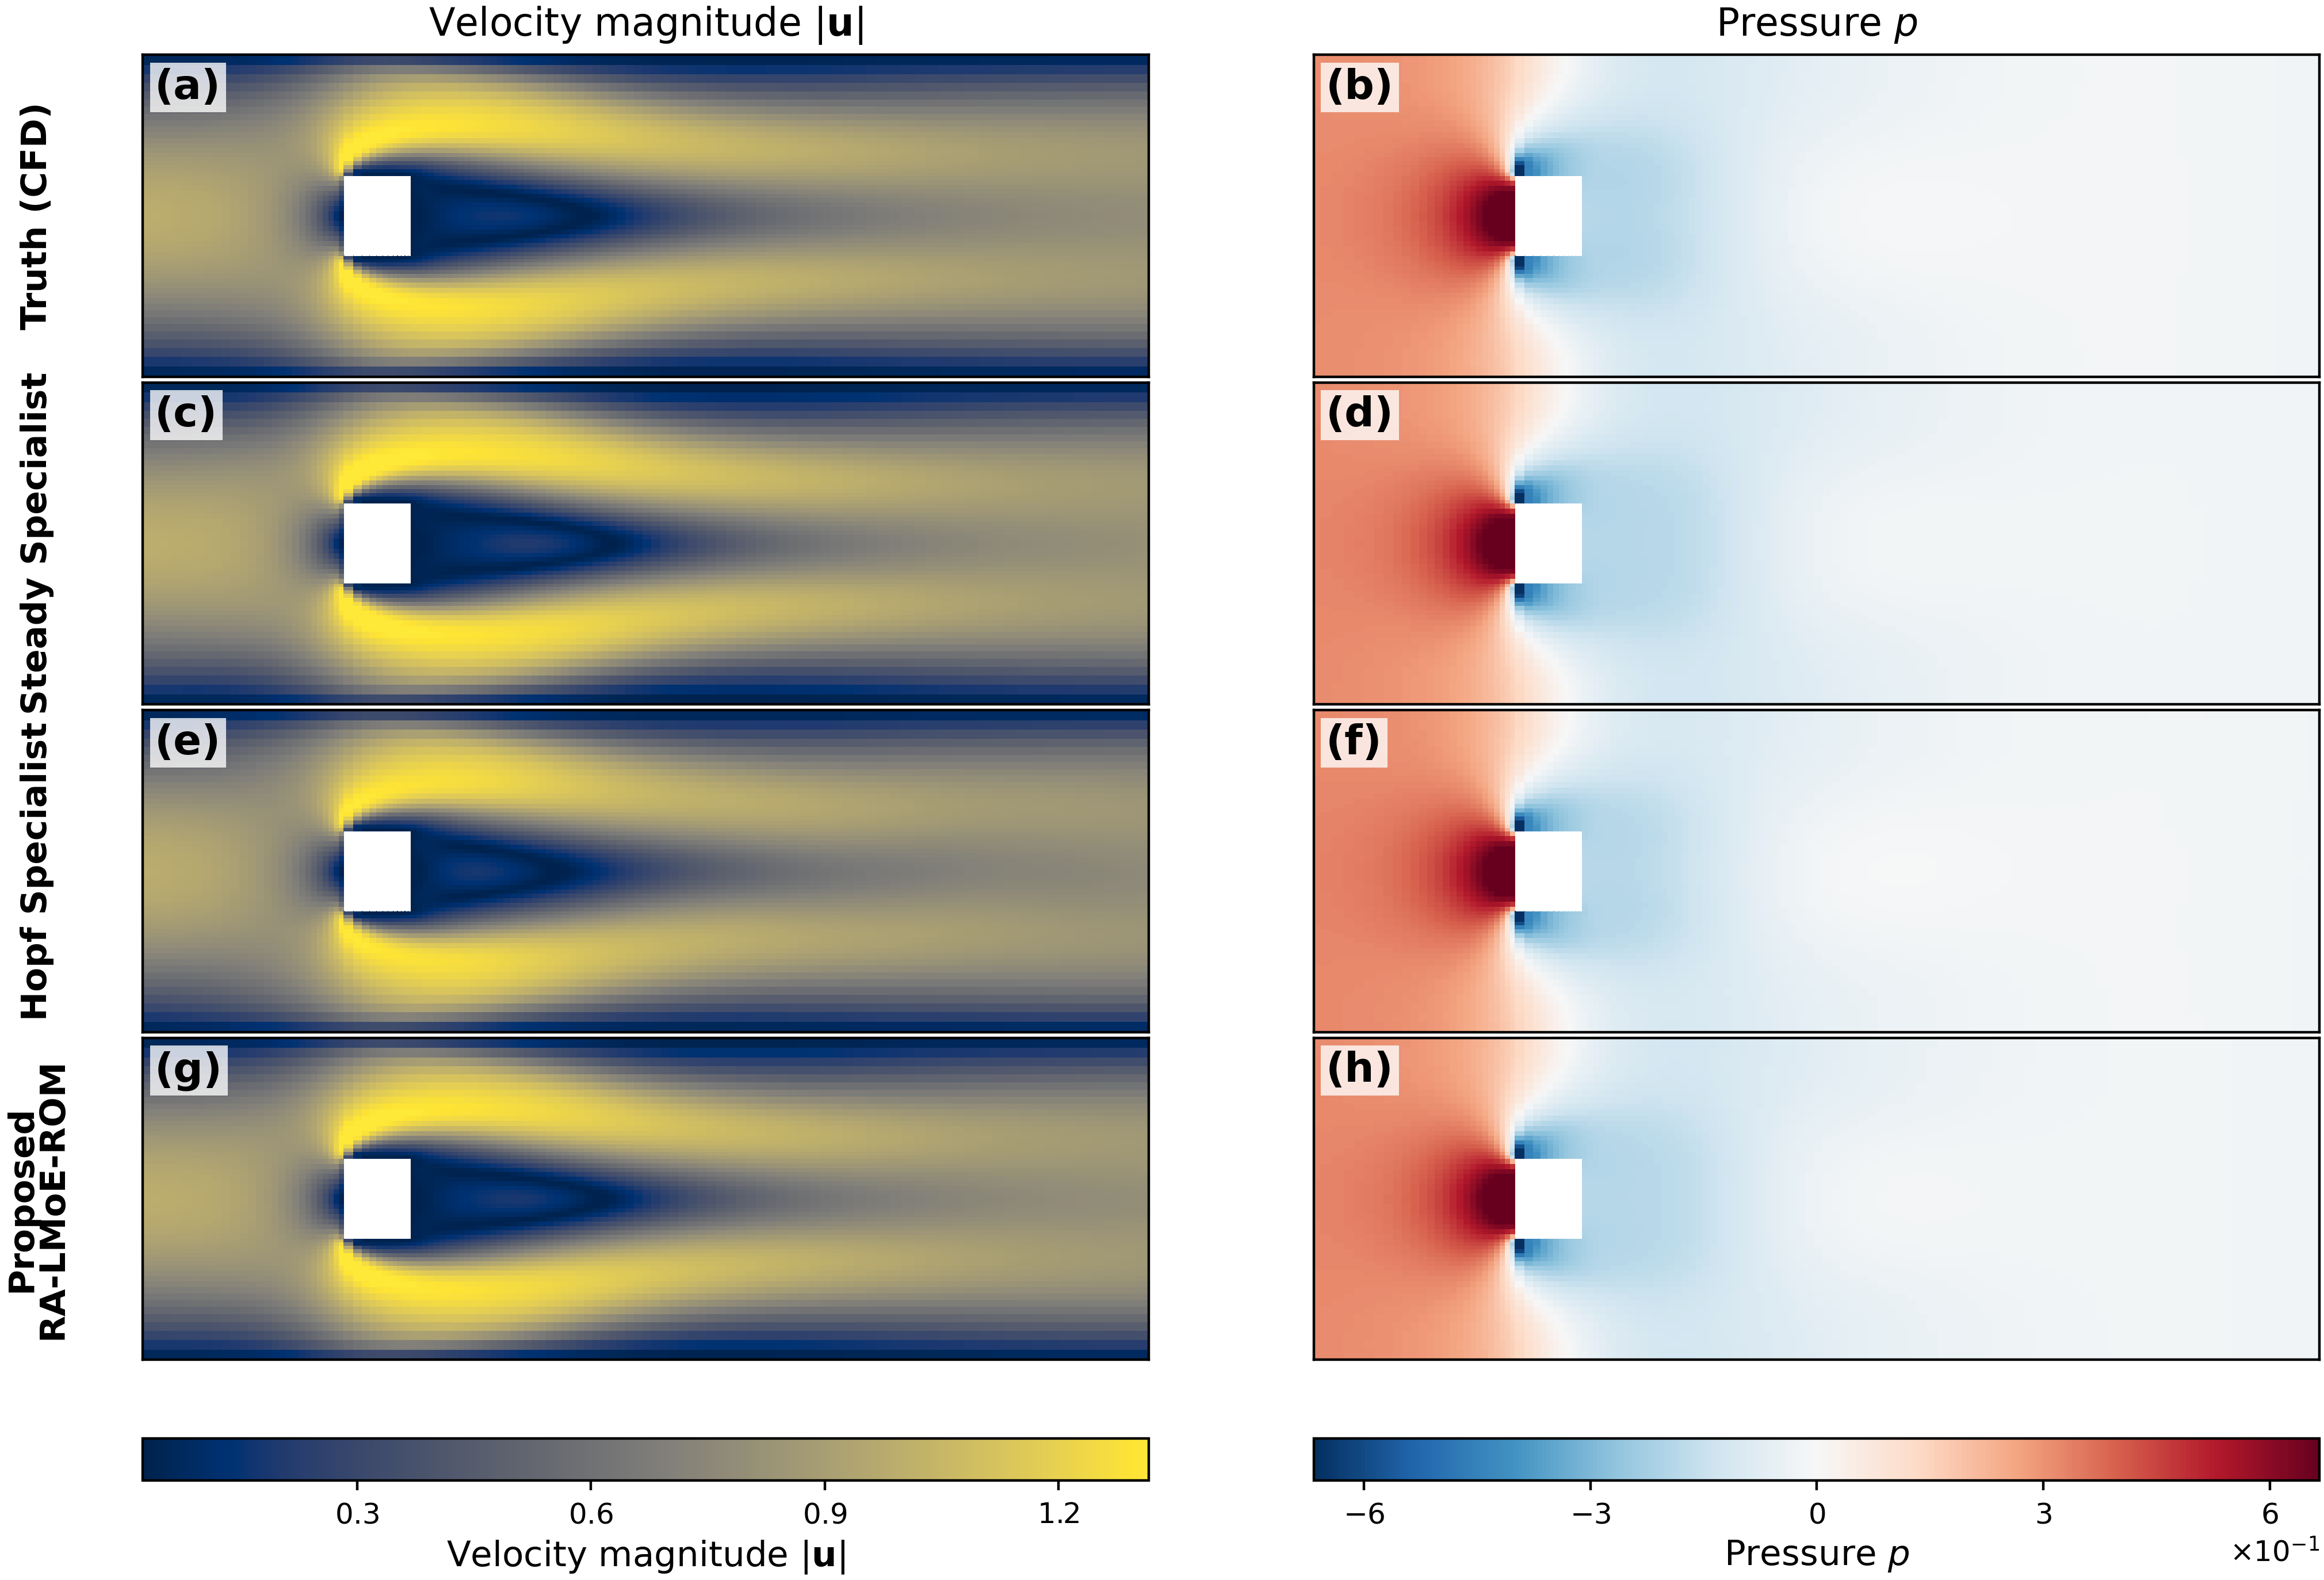
\includegraphics[width=0.80\linewidth]{figures/original/SH_2.png}

\vspace{0.35em}
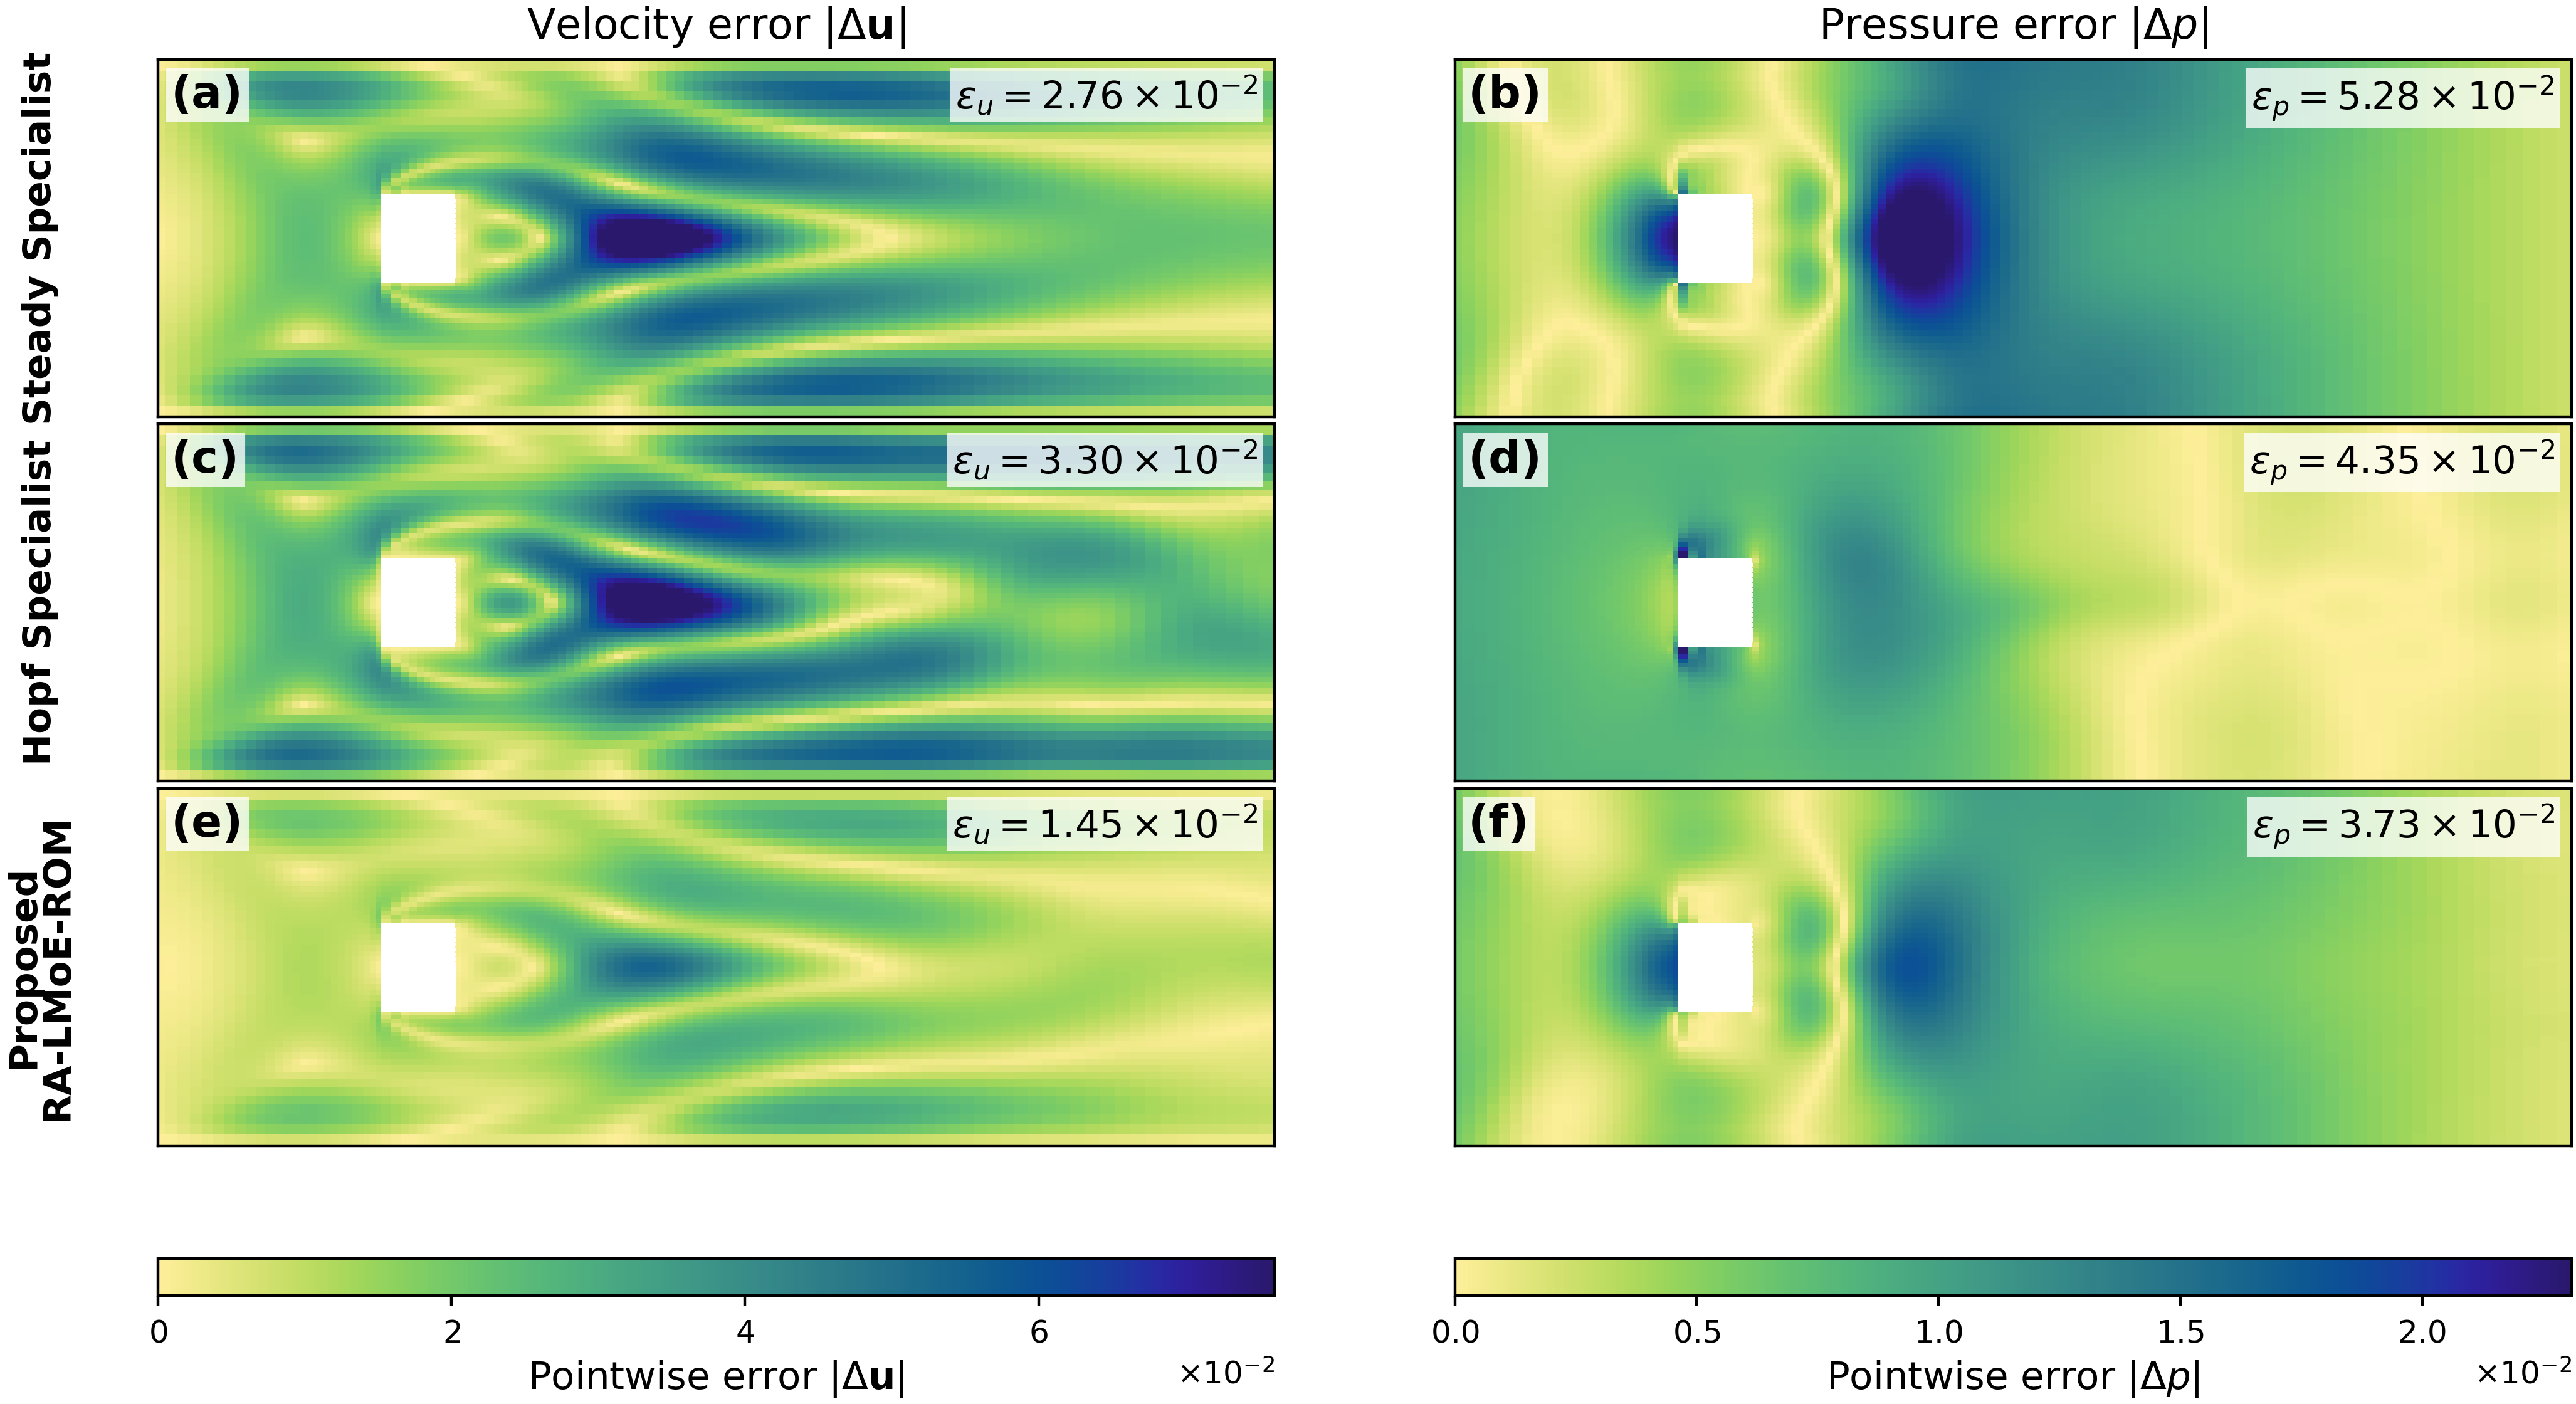
\includegraphics[width=0.80\linewidth]{figures/original/SH_2_1.png}
\caption{Representative held-out prediction in the centered-square
$S$--$H$ overlap at $Re=95.1$. The upper panel compares the CFD reference,
Steady specialist, Hopf specialist, and T2-C prediction for velocity
magnitude and gauge-corrected pressure. The lower panel gives the
corresponding pointwise absolute errors.}
\label{fig:app_square_sh_full}
\end{figure}

\begin{figure}[p]
\centering
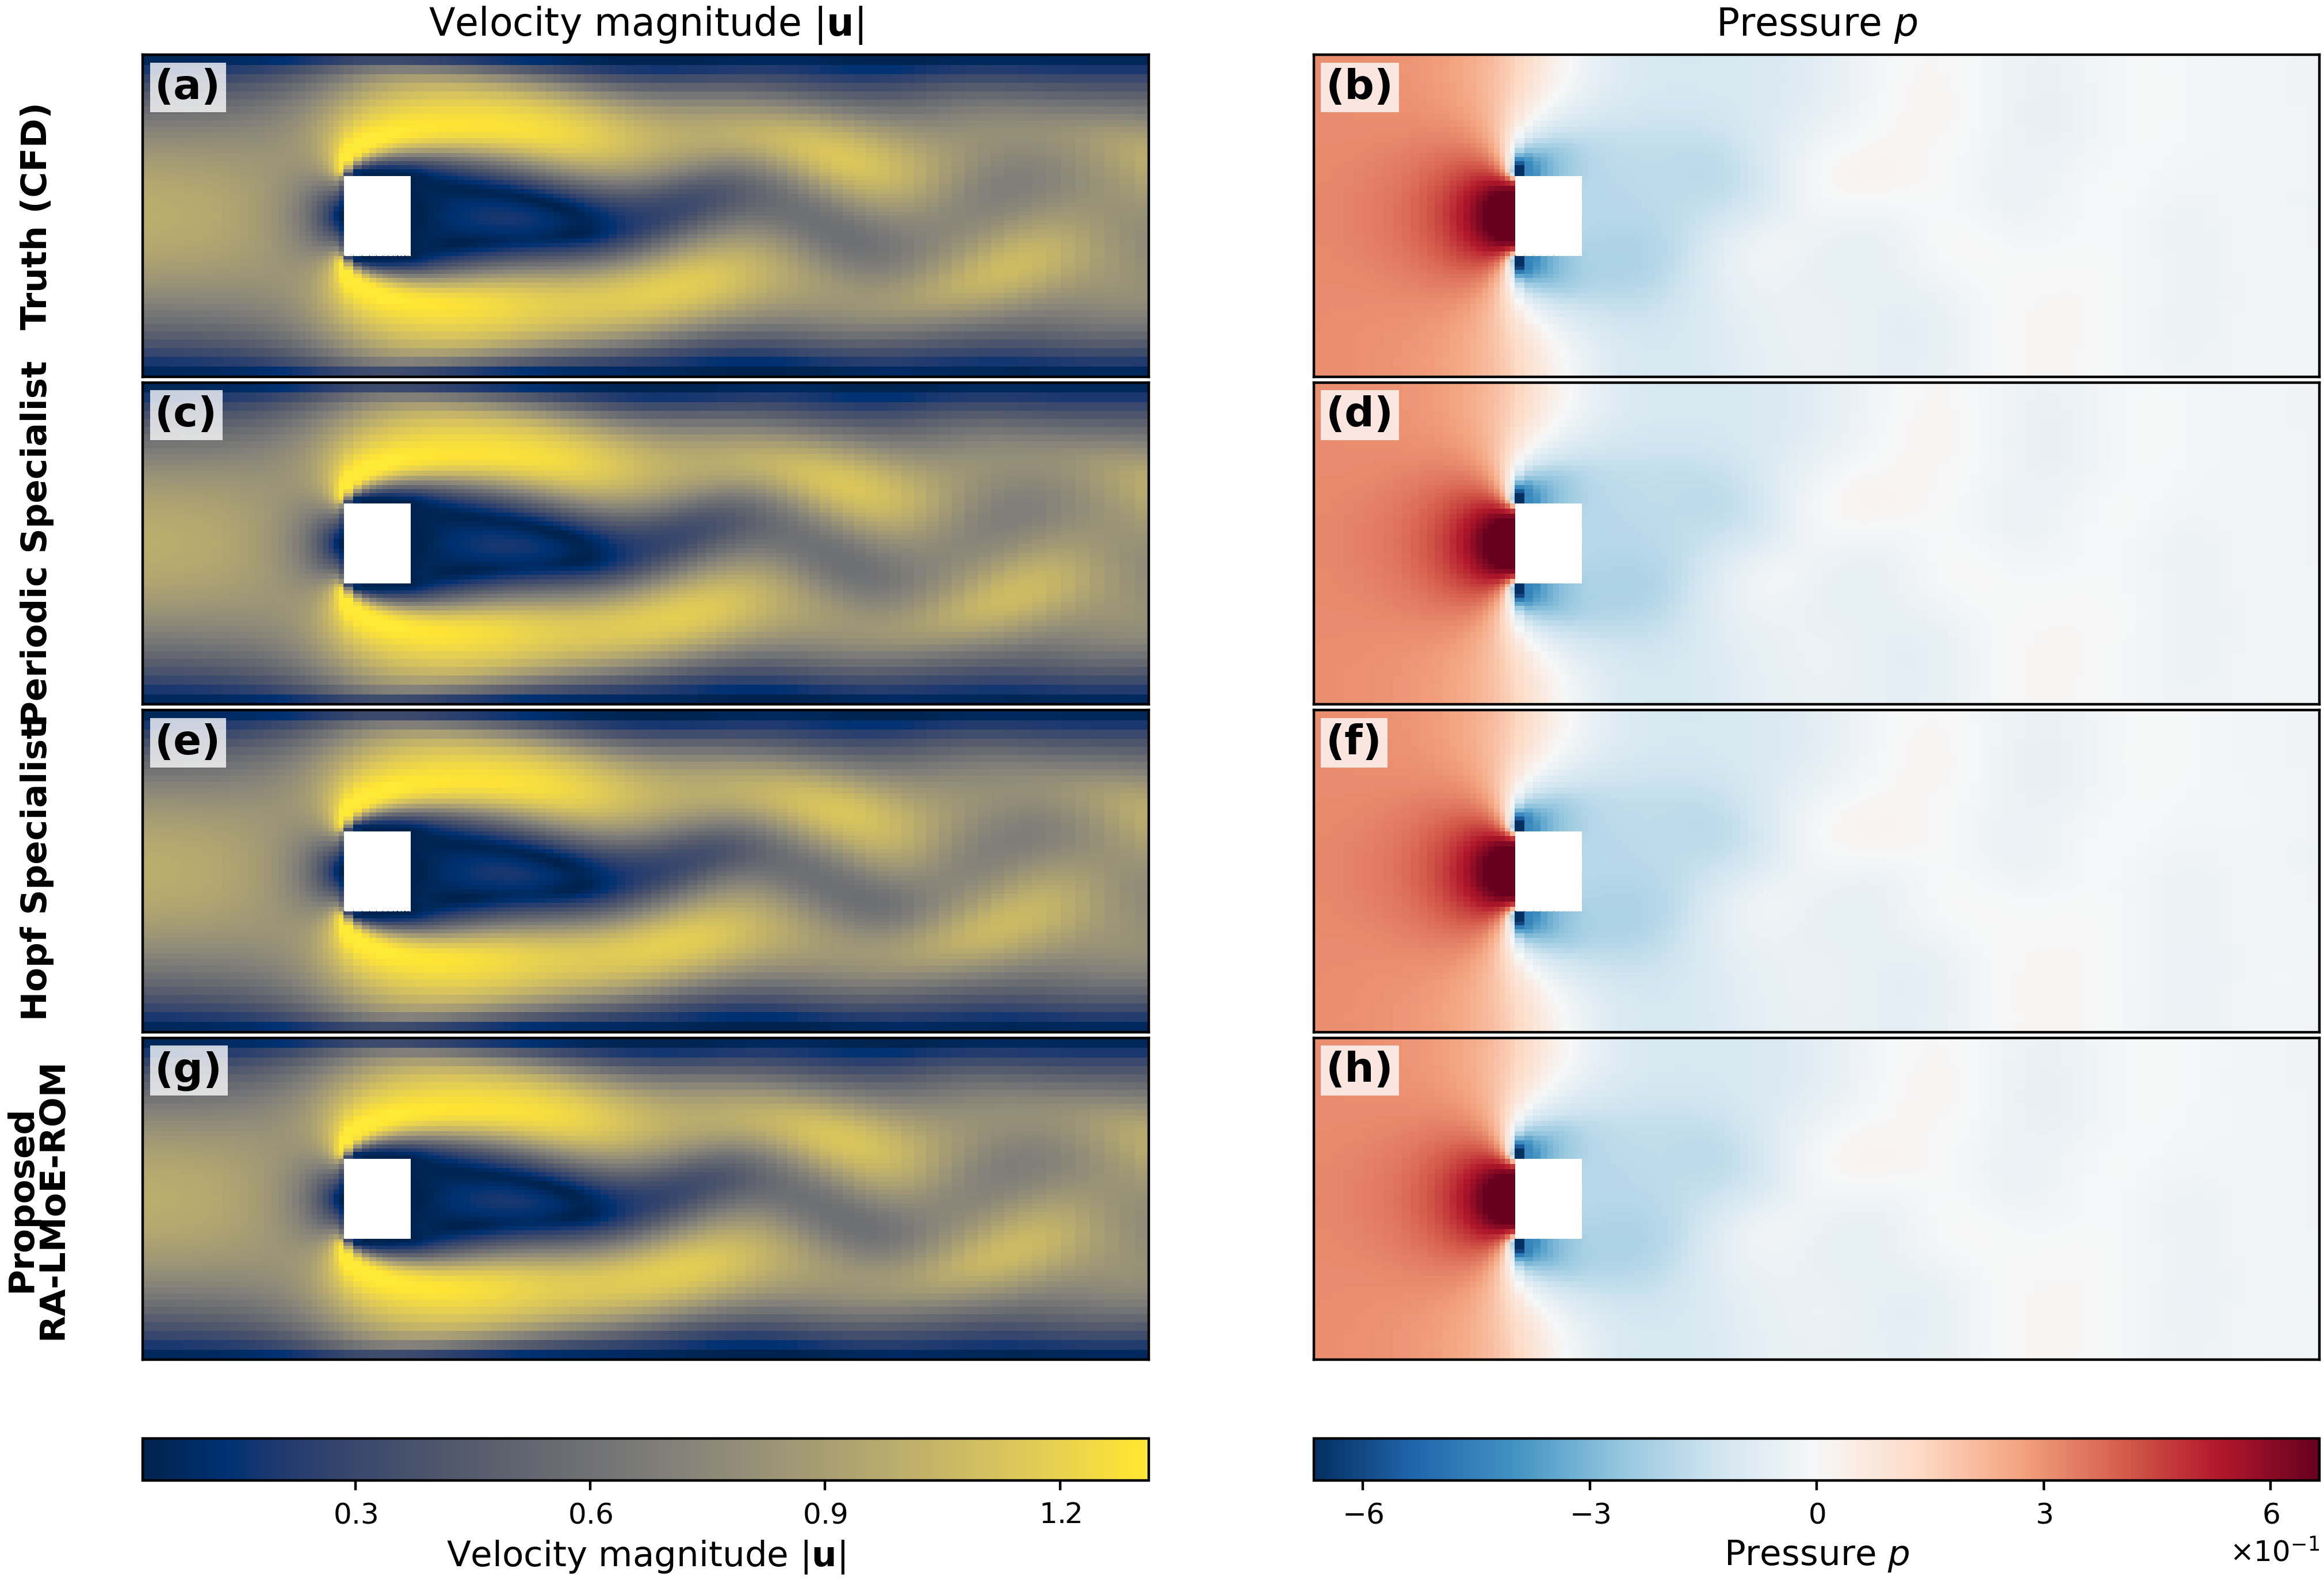
\includegraphics[width=0.80\linewidth]{figures/original/HP_2.png}

\vspace{0.35em}
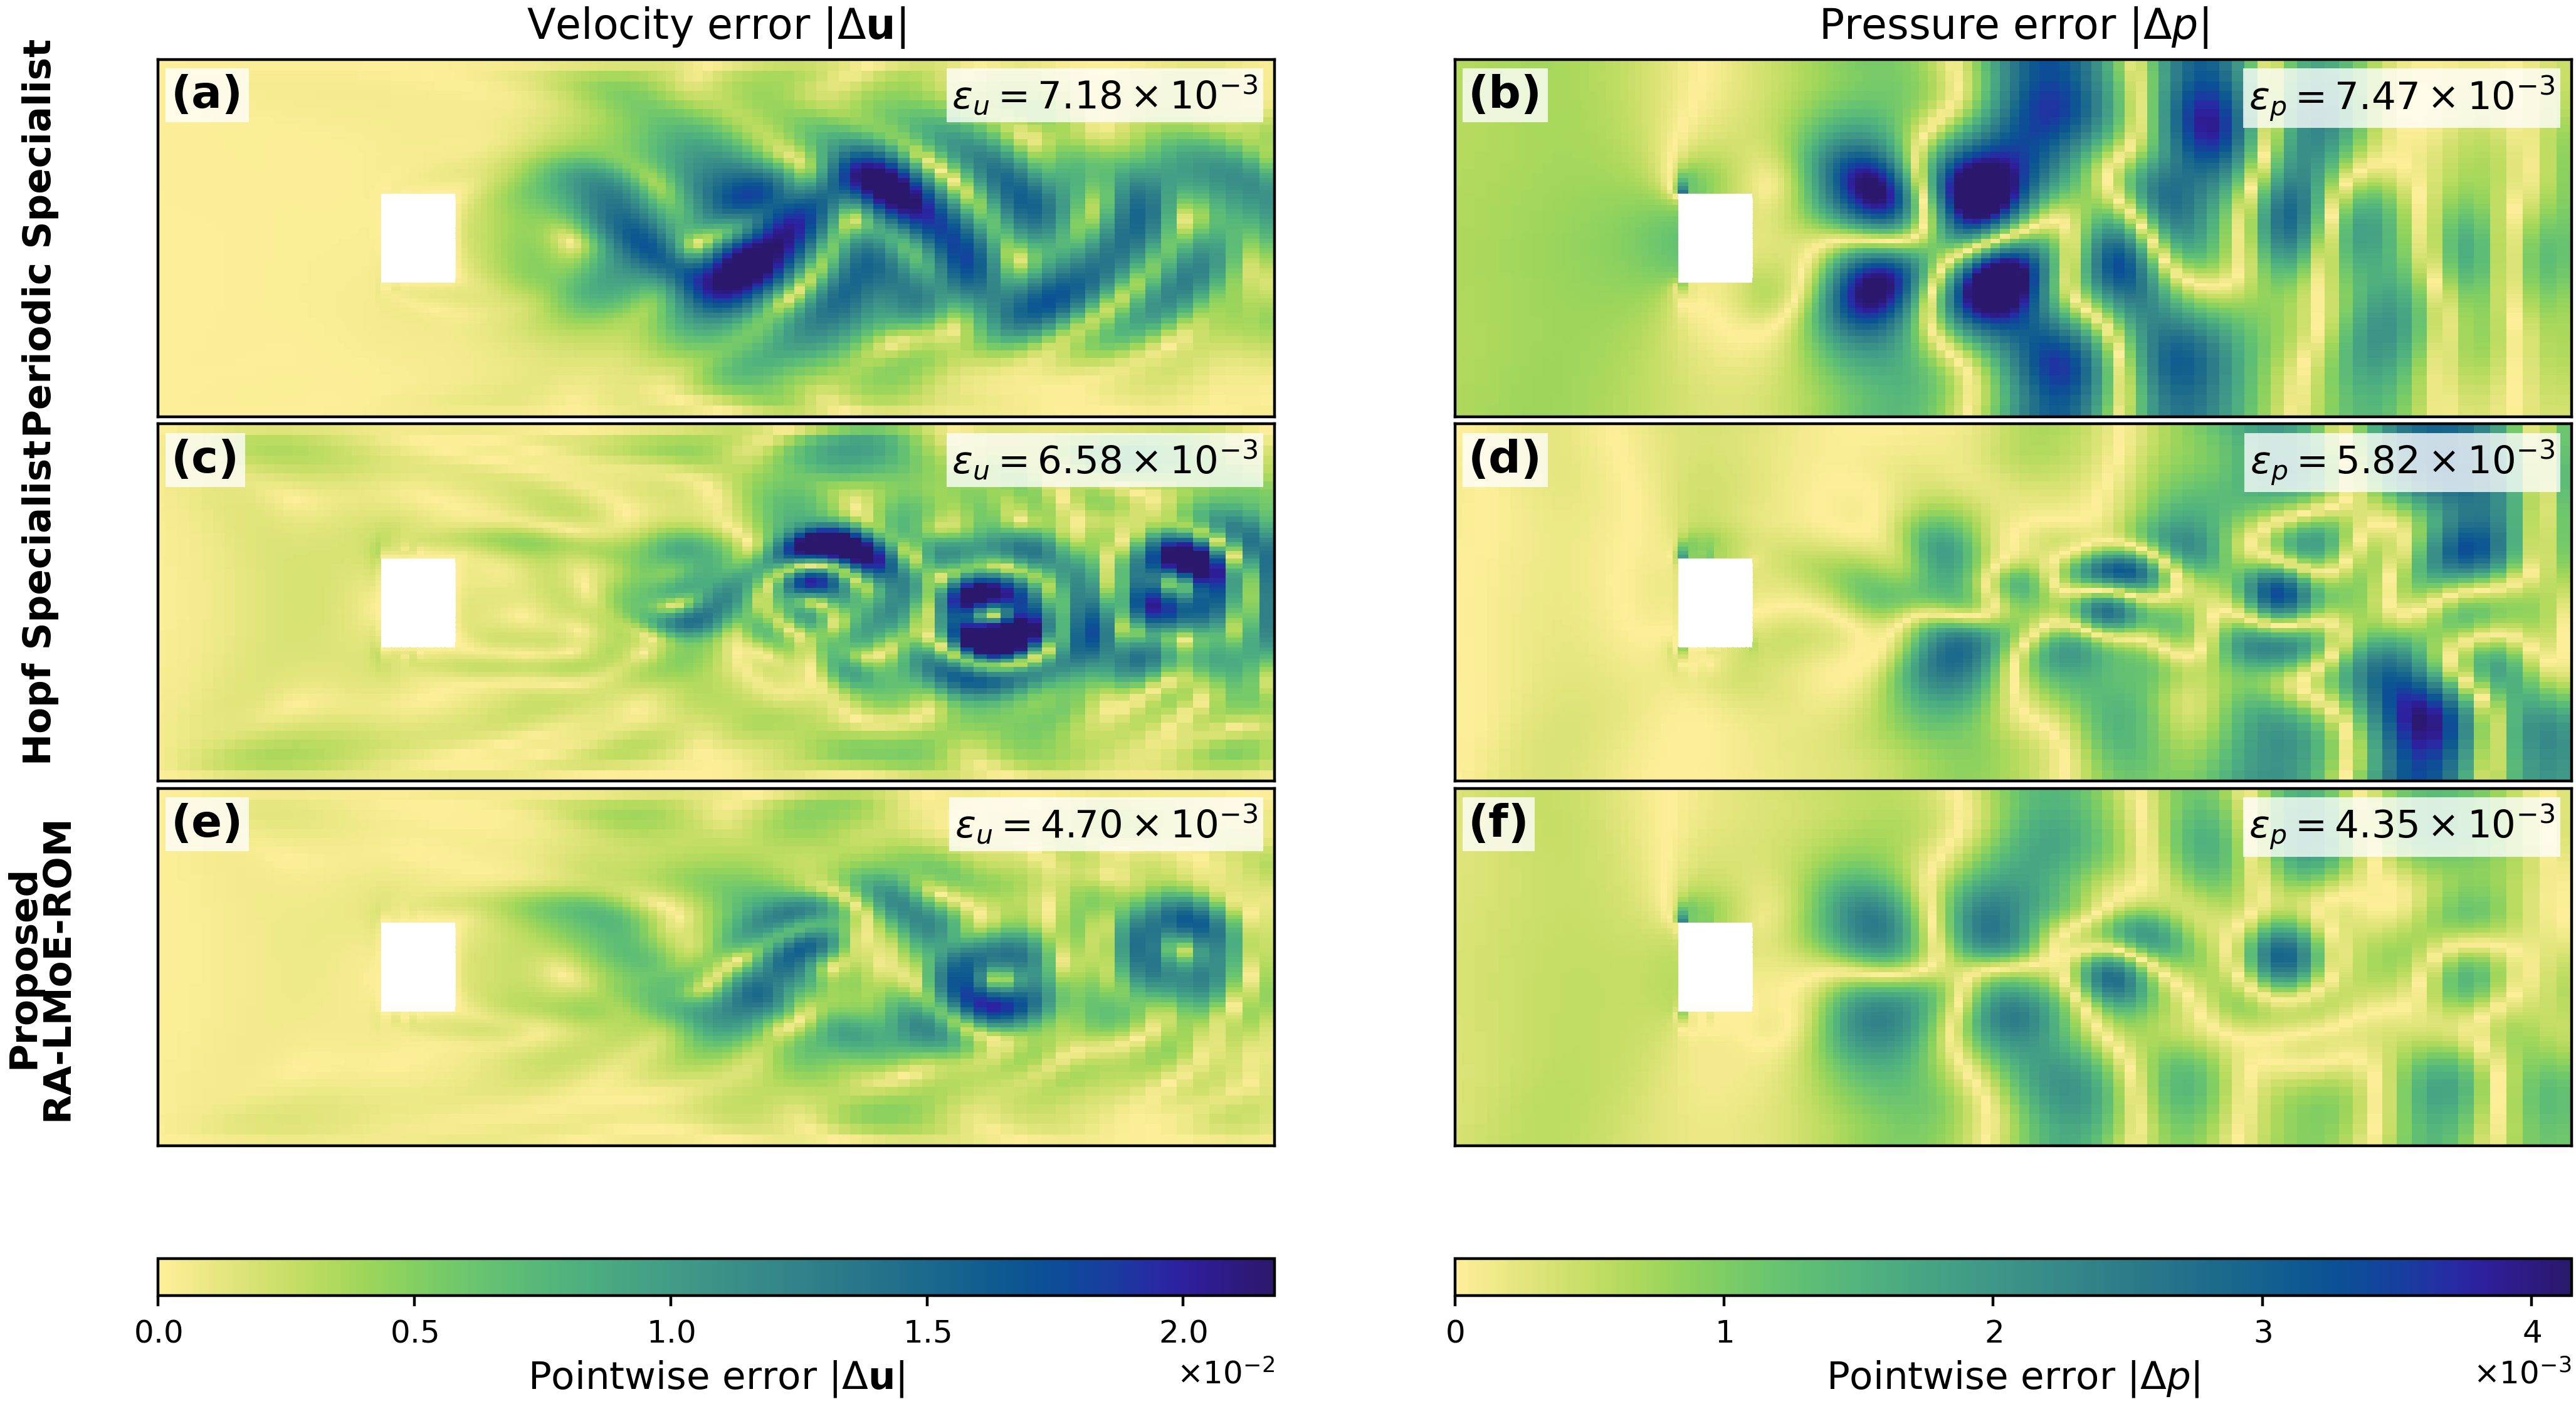
\includegraphics[width=0.80\linewidth]{figures/original/HP_2_1.png}
\caption{Representative held-out prediction in the centered-square
$H$--$P$ overlap at $Re=100.5$. The upper panel compares the CFD reference,
Periodic specialist, Hopf specialist, and T2-C prediction for velocity
magnitude and gauge-corrected pressure. The lower panel gives the
corresponding pointwise absolute errors.}
\label{fig:app_square_hp_full}
\end{figure}

\FloatBarrier
\section{Fluidic-pinball results}
\label{app:pinball}

The fluidic-pinball dataset contains 131 trajectories over $Re\in[10,60]$, with 94/19/18 train/validation/test trajectories overall. A POD--DeepONet one-step baseline gives $E_u=1.5921\%$ and $E_p=23.3447\%$ on 4,228 held-out input--output pairs, but only 1 of 28 held-out trajectories remains finite under recursive rollout. This contrast motivates evaluation under autonomous use rather than one-step accuracy alone. The one-step baseline uses a different cadence from the matched Periodic specialist evaluation and is not a cadence-matched long-horizon accuracy baseline.

\paragraph{Periodic-core evaluation protocol.}
The $K=32$ Periodic row in Table~\ref{tab:pinball_autonomous} reports the
standard periodic evaluation. Periodic core is the Periodic regime's core
final-test evaluation at $K=56$, using stride-four matched periodic chains.
Snapshots are stored every $0.25$ time units; taking every fourth snapshot
gives an effective sampling interval $\Delta t=1$. This aligns the evaluation
with the Periodic specialist's native history cadence and provides a
longer-horizon autonomous comparison within the same regime.

\begin{table}[h]
\centering
\caption{Fluidic-pinball overlap joint errors (\%). Primary denotes the Steady
specialist for $S$--$H$ and the Periodic specialist for $H$--$P$; the adjacent
specialist is Hopf in both cases. The oracle selects its convex weight a
posteriori for each evaluation window and is unavailable during prediction.}
\label{tab:pinball_overlap}
\small
\setlength{\tabcolsep}{3.5pt}
\begin{tabular}{lrccccc}
\toprule
Overlap & $K$ & Primary & Adjacent & E2 prob. & T2-C & Oracle \\
\midrule
$S$--$H$ & 24 & 0.6014 & 3.1925 & 1.7511 & 0.5897 & 0.5889 \\
$S$--$H$ & 56 & 0.6927 & 3.1193 & 1.7714 & 0.6767 & 0.6763 \\
$H$--$P$ & 24 & 0.0990 & 0.5146 & 0.2972 & 0.0945 & 0.0928 \\
$H$--$P$ & 56 & 0.1028 & 0.5346 & 0.3085 & 0.0978 & 0.0955 \\
\bottomrule
\end{tabular}
\end{table}

T2-C improves the primary single-specialist prediction in all four overlap evaluations and remains close to the window-wise convex oracle. The result is consistent across the short and long rollout horizons shown here.

\FloatBarrier
\section{Additional internal-routing diagnostics}
\label{app:internal_routing}

\paragraph{Evaluation and statistics.}
We inspect the fixed circular-cylinder Hopf and Periodic specialists on their
held-out autonomous rollout windows. The Periodic analysis uses 13 fixed windows
at each of four held-out Reynolds numbers ($52$ windows, $K=48$); the Hopf
analysis uses five fixed windows at each of three held-out Reynolds numbers
($15$ windows, $K=56$). Each statistic uses one routing record per macro-step,
taken at its first integration stage, giving $2496$ Periodic and $840$ Hopf
decisions per channel. These are macro-step statistics, not a count of all
right-hand-side evaluations. Overlapping windows are not treated as independent
trajectories, and no diagnostic is used for model selection.

For $N$ decisions, let $I_{n,e}$ indicate whether routed expert $e$ is selected,
with group identity included in $e$. We report normalized activation frequency
$f_e=\sum_n I_{n,e}/(2N)$ and mean routing mass
$m_e=N^{-1}\sum_n\omega_{n,e}I_{n,e}$, retaining zero-use experts.
The utilization entropy is
$H=-\sum_{e:f_e>0}f_e\log f_e/\log N_E$, where $N_E$ counts all routed
experts in the corresponding channel. Distinct pairs include group identity
but ignore the order of the two selected experts. The shared/routed mixture
coefficient is fixed by architecture; a shared expert is always active in the
selected group, while the routed component is allocated conditionally.
For both specialists here, the shared coefficient is $4/7$ and
$\sum_e m_e=3/7$.
Routing mass is a mixing coefficient, not the norm of an expert's output or
its causal contribution to prediction.
Figure identifiers such as \texttt{g0:e0} enumerate routed experts only;
they are distinct from the shared-expert index $0$ in
Eq.~(\plaineqref{eq:app_channel_sparse_moe}).

\begin{table}[htbp]
\centering
\caption{Post-hoc internal-routing statistics on held-out autonomous rollout
windows. Entropy is a descriptive utilization statistic, not a performance
score. A fixed Top-2 pair has nonzero entropy; the two specialists also have
different numbers of available groups.}
\label{tab:internal_routing_summary}
\small
\setlength{\tabcolsep}{5pt}
\begin{tabular}{@{}llrrrr@{}}
\toprule
Specialist & Channel & Used experts & Distinct pairs & Dominant pair (\%) & $H$ \\
\midrule
Hopf & Velocity & 2/6 & 1 & 100.00 & 0.387 \\
     & Pressure & 2/6 & 1 & 100.00 & 0.387 \\
\addlinespace
Periodic & Velocity & 18/18 & 33 & 16.27 & 0.929 \\
         & Pressure & 14/18 & 16 & 31.25 & 0.784 \\
\bottomrule
\end{tabular}
\end{table}

\paragraph{Hopf routing profile.}
The Hopf specialist exhibits a different sparse-routing pattern from the
Periodic model. It contains one group by construction and selects a fixed
channel-specific pair over the evaluated windows: $(e_1,e_3)$ for velocity
and $(e_2,e_4)$ for pressure. The same selected pairs occur at all four
integration stages. Velocity expert $e_3$ accounts for approximately
$99.93\%$ of pooled routed mass; pressure expert $e_2$ accounts for
$84.16\%$. The pressure pair nevertheless retains variable internal
weighting: the mean mass assigned to the secondary pressure expert $e_4$
increases markedly across the three held-out Reynolds numbers.
Thus, routing profiles are chart dependent: Periodic uses a broad set of
configurations, whereas Hopf uses stable sparse support with nonuniform
mixing weights. The sole Hopf group is a structural choice, not evidence of
competition collapsing among multiple groups.

\paragraph{Periodic rollout-position diagnostic.}
Figure~\ref{fig:periodic_routing_step} reports routed-expert mass as a function
of normalized rollout position, pooling the same 52 fixed held-out windows.
This is a temporal routing diagnostic, not an estimate of physical oscillation
phase. Together with Figure~\ref{fig:periodic_internal_routing}, it describes
conditional allocation within the Periodic specialist without assigning
physical semantics to expert identities.

\begin{figure}[htbp]
\centering
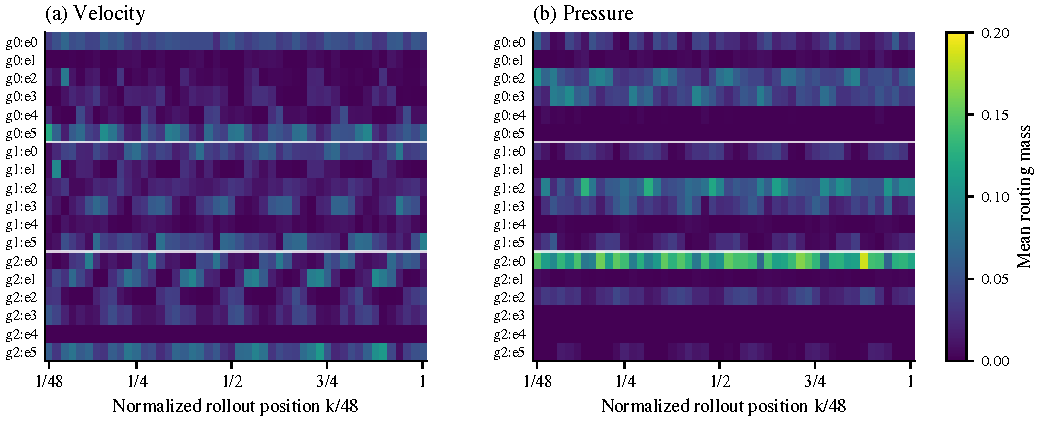
\includegraphics[width=\linewidth]{figures/periodic_rollout_step_routing.pdf}
\caption{Routing mass across autonomous rollout position for the
circular-cylinder Periodic specialist. Each column averages the corresponding
macro-step decision over the fixed held-out windows; all routed-expert rows
are retained. The horizontal coordinate denotes normalized rollout position
$k/48$ and is not interpreted as physical oscillation phase.}
\label{fig:periodic_routing_step}
\end{figure}

\clearpage
\section{Trainable and active parameter counts}
\label{app:parameter_counts}

\paragraph{Counting convention.}
Total parameters count unique trainable parameters in each analyzed
circular-cylinder specialist. Active parameters count unique trainable
parameters used by one batch-size-one prediction-path routing decision,
not their union across a batch, trajectory, or all RK4 stages. These include
the encoder and refinement blocks, executed routers, the selected group's
shared experts, channel-specific Top-2 velocity and pressure experts, and
the learned pressure correction. Fixed POD bases, projected operators,
normalization statistics, and non-trainable buffers are excluded.

\begin{table}[htbp]
\centering
\caption{Trainable and per-decision active parameter counts for the analyzed
circular-cylinder specialists. Active counts refer to the sparse prediction
path; M denotes one million parameters.}
\label{tab:parameter_counts}
\begin{tabular}{lrrr}
\toprule
Specialist & Total trainable & Active prediction & Active fraction \\
\midrule
Hopf & 31.81M & 14.17M & 44.53\% \\
Periodic & 48.62M & 8.31M & 17.09\% \\
\bottomrule
\end{tabular}
\end{table}

The Hopf and Periodic specialists activate 44.53\% and 17.09\% of their
trainable parameters per prediction decision, respectively. These counts
describe conditional parameter activation, not measured FLOPs, runtime,
or speedup. Complete parameter-matched counts are unavailable for the
Vanilla-FNN-MoE, DataOnly-MoE, and Global MoE ablations, so the local
architecture comparison is not interpreted as a capacity-matched study.


\end{document}
